\documentclass[11pt,letterpaper]{article}
\input{headings}
\newcommand \recipeName {Risolis}
\newcommand \fileName {Risolis}
\chead{\recipeName}

\begin{document}
\input{title}

This is a very flavourful finger food dish that is best served warm with a cold beer or a cold lemonade. This is a Brazilian classic dish and it is found all over the country. This is my mother's version and it is very well regarded. In Brazil the recipe calls for one cup of milk. In Alberta the weather is very dry and thus the flour is quite dry. Thus I have increased the amount of milk to 1 1/4 cup.

Below is the classic version. You can make a dairy-free version  by replacing the milk for water and the butter for margarine. There are many variations for the filling: beef with tomato sauce; lightly sauteed shrimp ground up, mushroom duxelles with heavy cream, a combination of good melting cheeses with dried herbs. The chicken filling itself can be flavoured in many ways with various fresh herbs. However, this classic version is my favourite.
 
\begin{description}

\item[Ingredients:]\ \\
	\begin{itemize}
	\item 1 1/4 cup of milk (10 3/4 oz = 305 grams)
	\item 1 1/2 cup of flour (7.5 oz = 212 grams)
	\item 1 Tablespoon of butter
	\item 1/2 teaspoon of salt
	\item 2 eggs
	\item 1 1/2 cups of freshly made bread crumbs
	\item 3 to 4 cups of flavourless cooking oil
	\item \href{ChickenFilling.html}{chicken filling}
	\end{itemize}

\item[Procedure:]\ \\
	\begin{enumerate}
	\item {\bf Make the dough}
	\begin{itemize}
	\item In a sauce pan boil the milk with the butter and salt.
        \item Once the milk is boiling, dump the flour at once into the boiling milk.
	\item Using a wooden spoon, mix the dough until it is releasing from the bottom of the pan.
	\item Let the dough cool until it is safe to handle.
	\end{itemize}
	\item {\bf Shape the risolis}
	\begin{itemize}
	\item Working with 1/3 of the dough at a time, keep the remainder dough covered with plastic wrap to avoid drying.
	\item Roll out the dough to a 1/16 of an inch.
	\item Using a water glass, cut circles of dough.
	\item Carefully spoon a small amount of feeling in the center of each circle.
	\item Fold each circle and press the edges together to close the risolis.
	\item Put each risolis in a covered dish to avoid drying.
	\end{itemize}
	\item {\bf Bread the risolis}
	\begin{itemize}
	\item Break the eggs into a dish and add a tablespoon of water.
	\item Add a small dash of salt.
	\item Beat the eggs until they are very well mixed.
	\item Put the bread crumbs in another dish.
	\item Working with a few at a time, deep the risolis in the egg wash and then coat with bread crumbs.
	\item If you will cook in the next couple of days, you can put the risolis in a covered dish and keep in the refrigerator.
	\item You can also freeze the risolis at this point. 
		\begin{itemize}
		\item Place the risolis spaced apart on a baking sheet lined with parchment paper.
		\item Put in the freezer.
		\item Once they are frozen you can put them in a ziplock plastic bag.
		\end{itemize}
	\end{itemize}
	\item {\bf Fry the risolis}
	\begin{itemize}
	\item Put the cooking oil in a sauce pan. The quantity depends on how many risolis you plan to fry and on the size of the saucepan. You need to have enough oil to submerge the risolis.
	\item Fry the risolis until they are golden. 
	\item Let the risolis cool off in a rack but serve them warm.
	\end{itemize}
	\end{enumerate}
\end{description}

\begin{table}
\begin{tabular}{cccc}
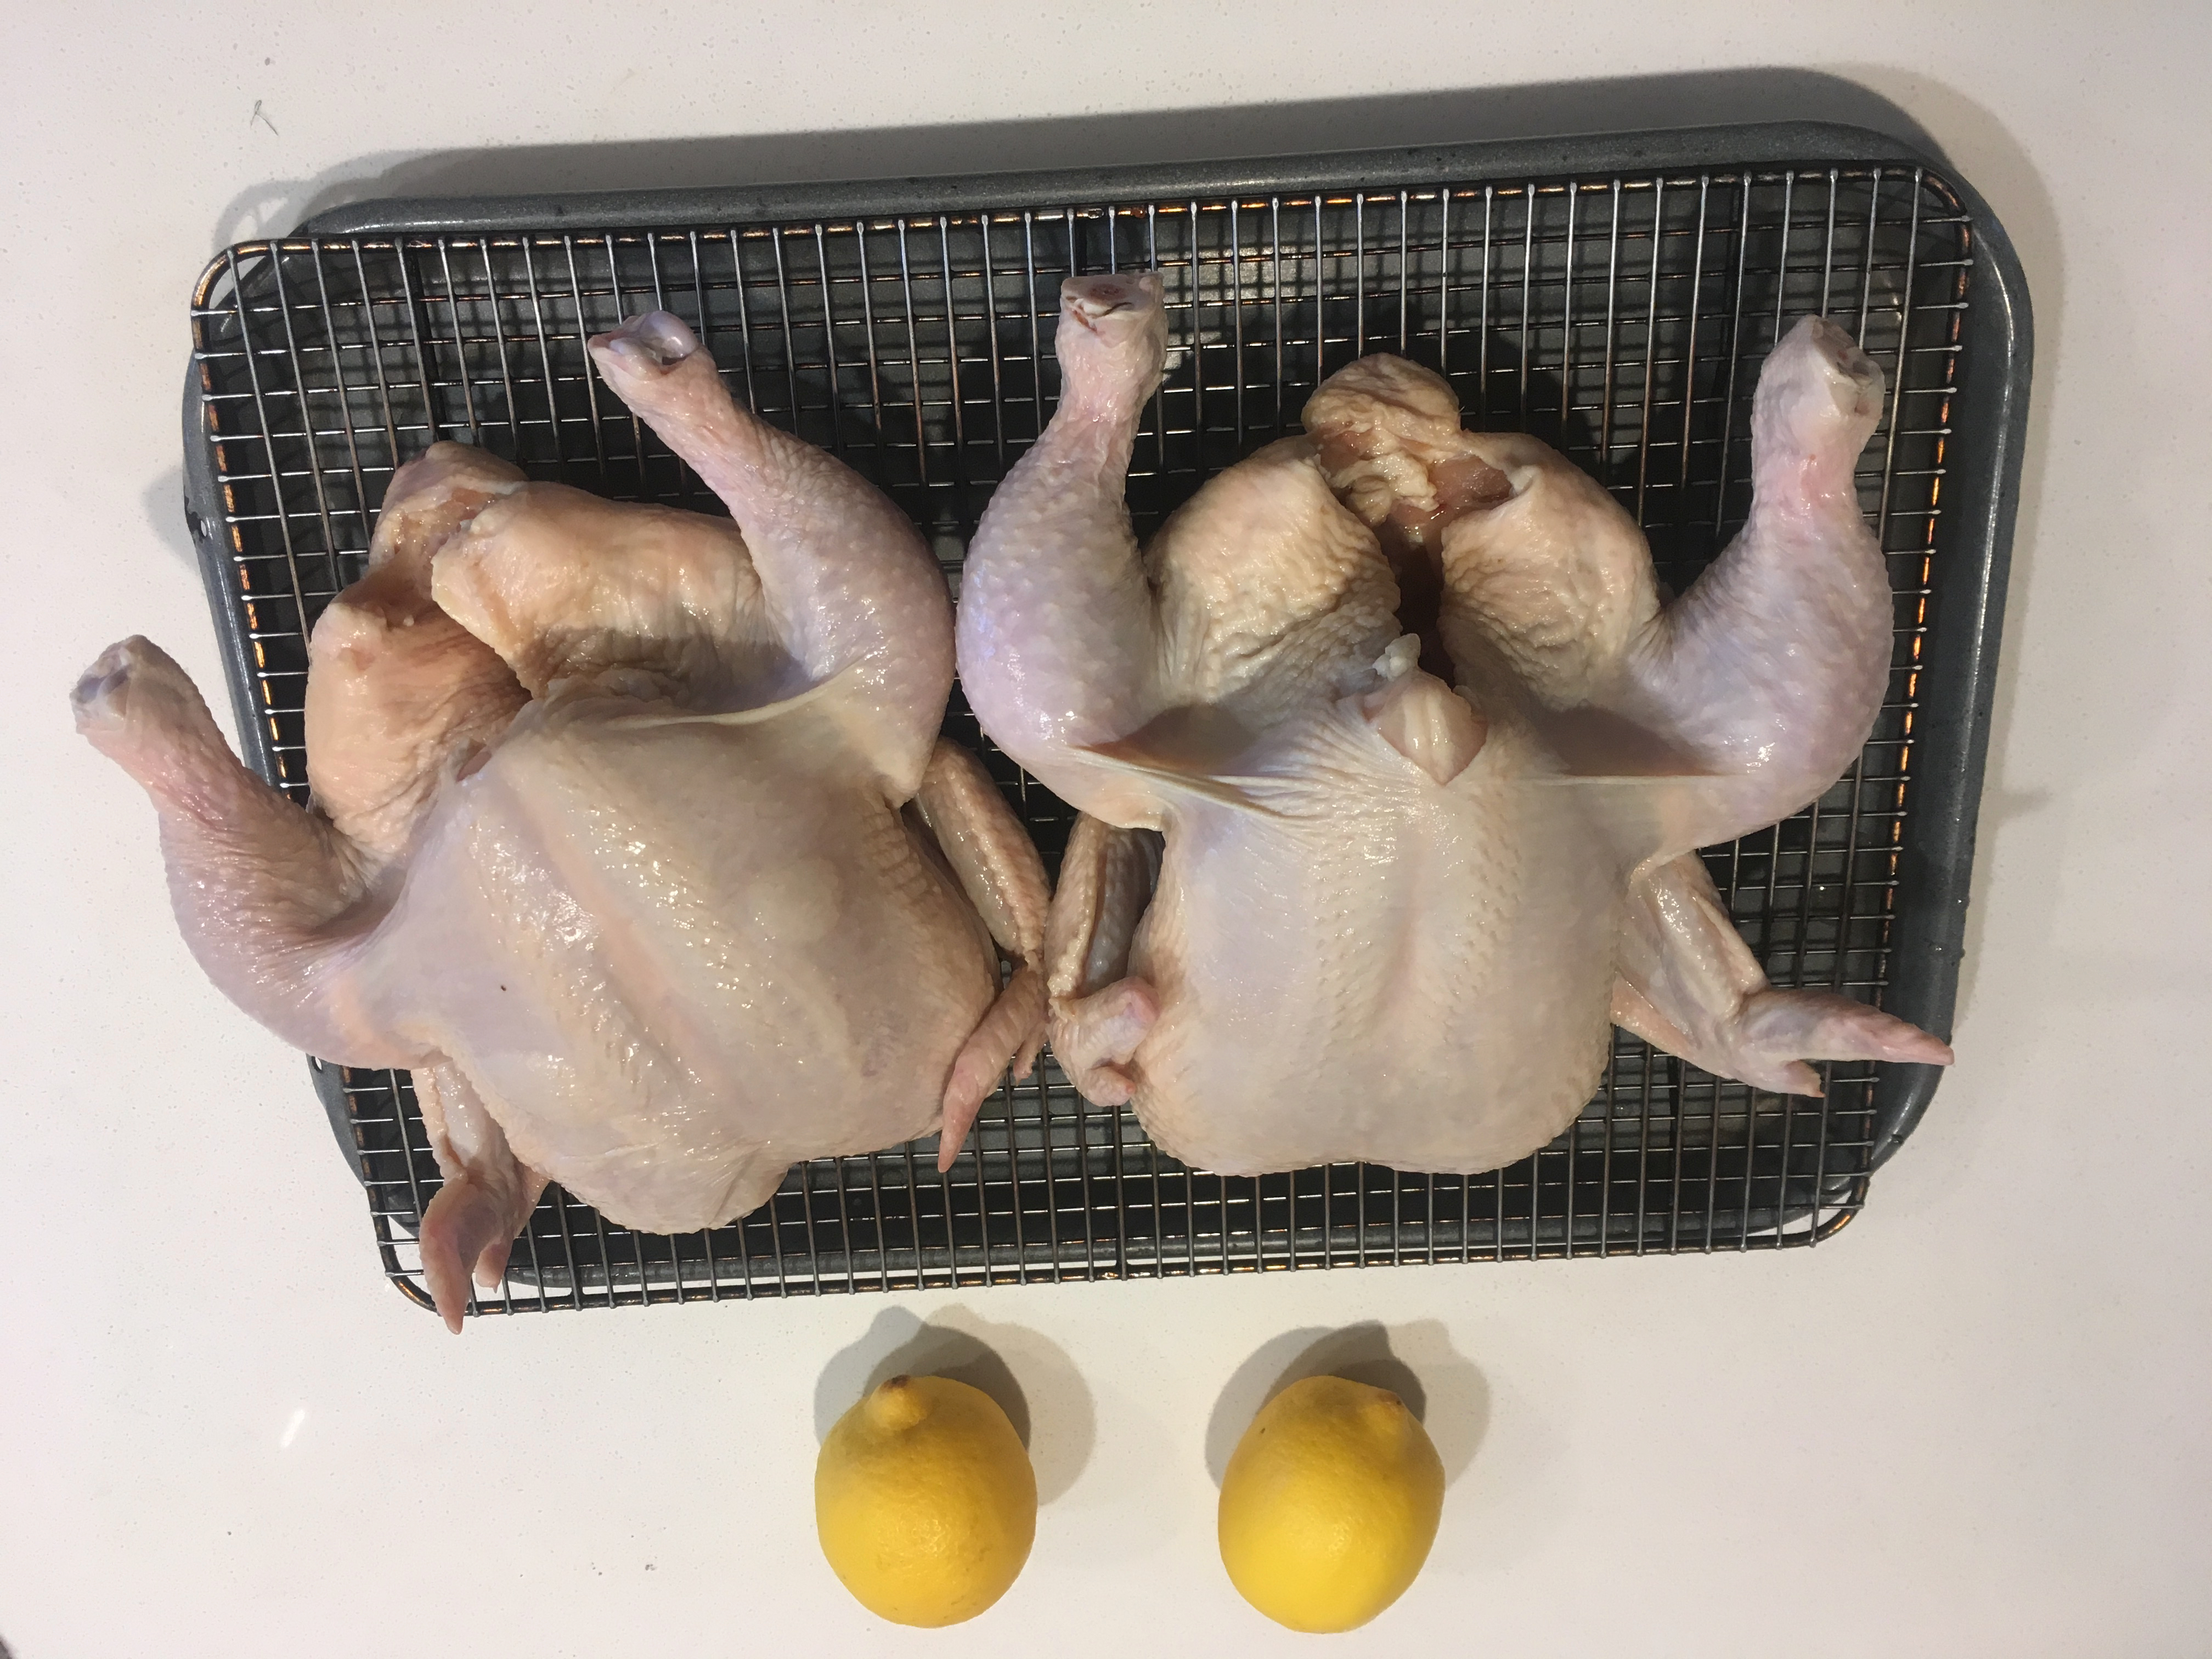
\includegraphics[width=0.25\textwidth]{\imageDir/\fileName/IMG_3197.jpg} &
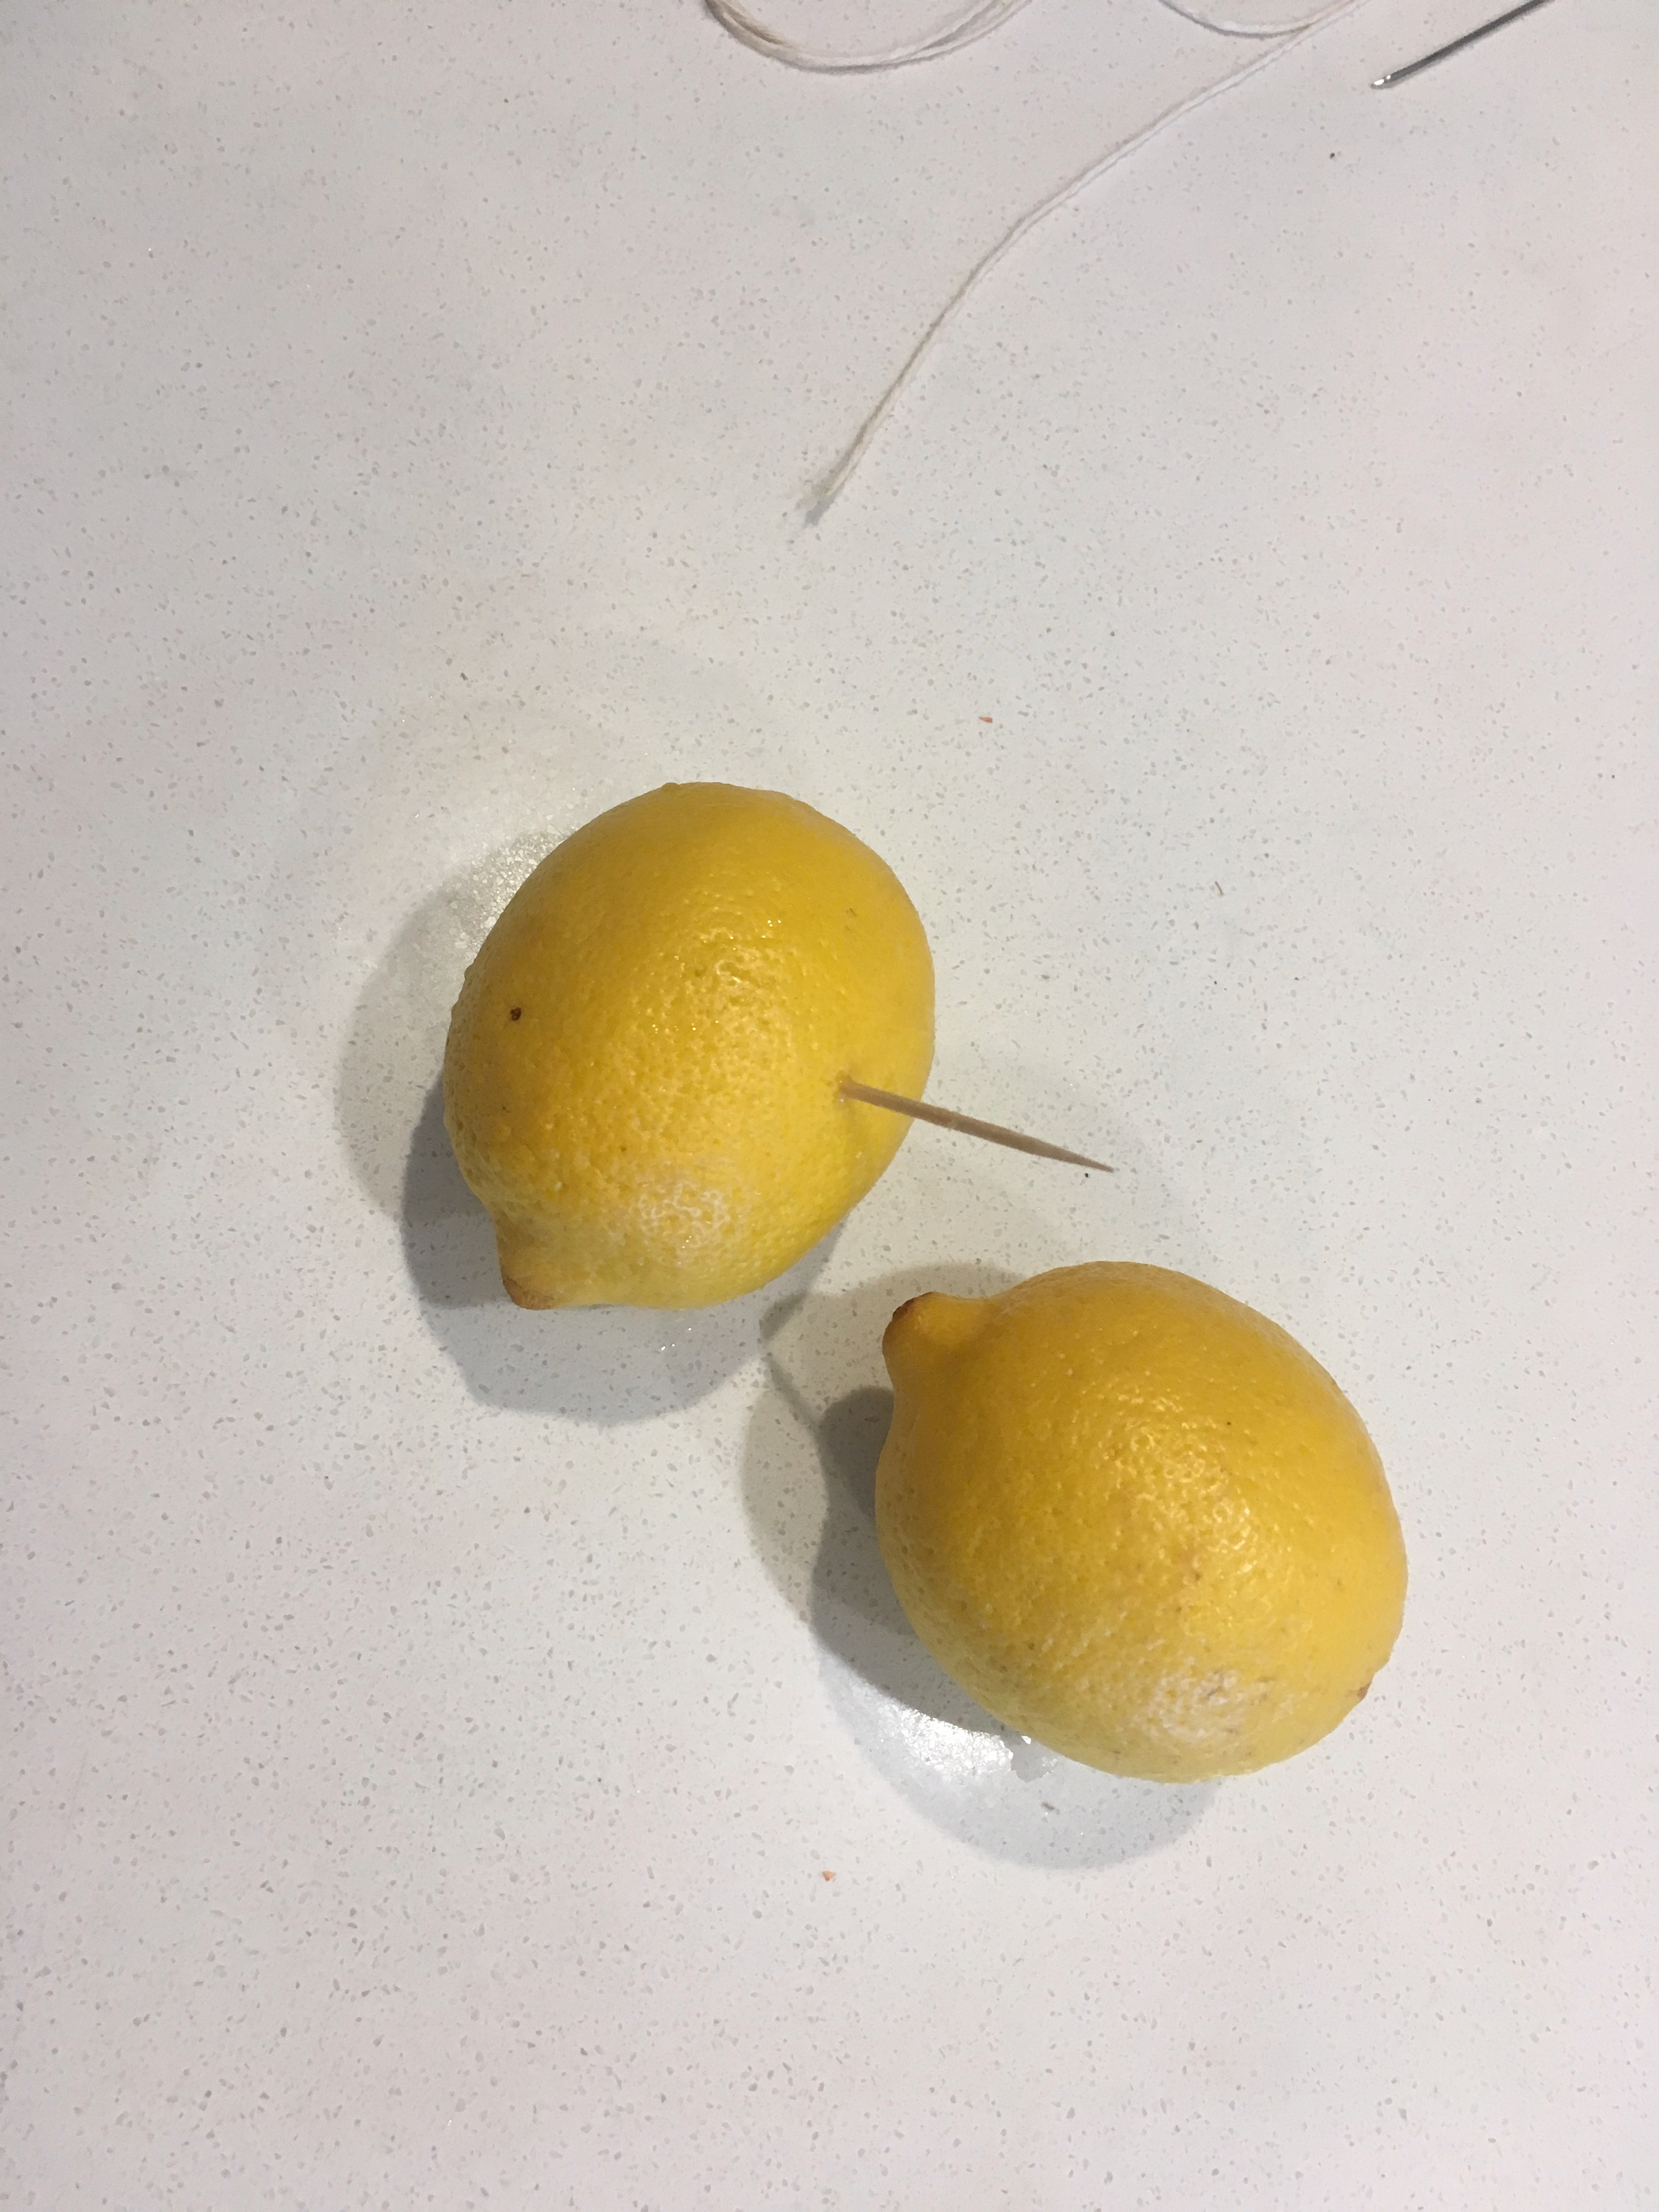
\includegraphics[width=0.25\textwidth]{\imageDir/\fileName/IMG_3212.jpg} &
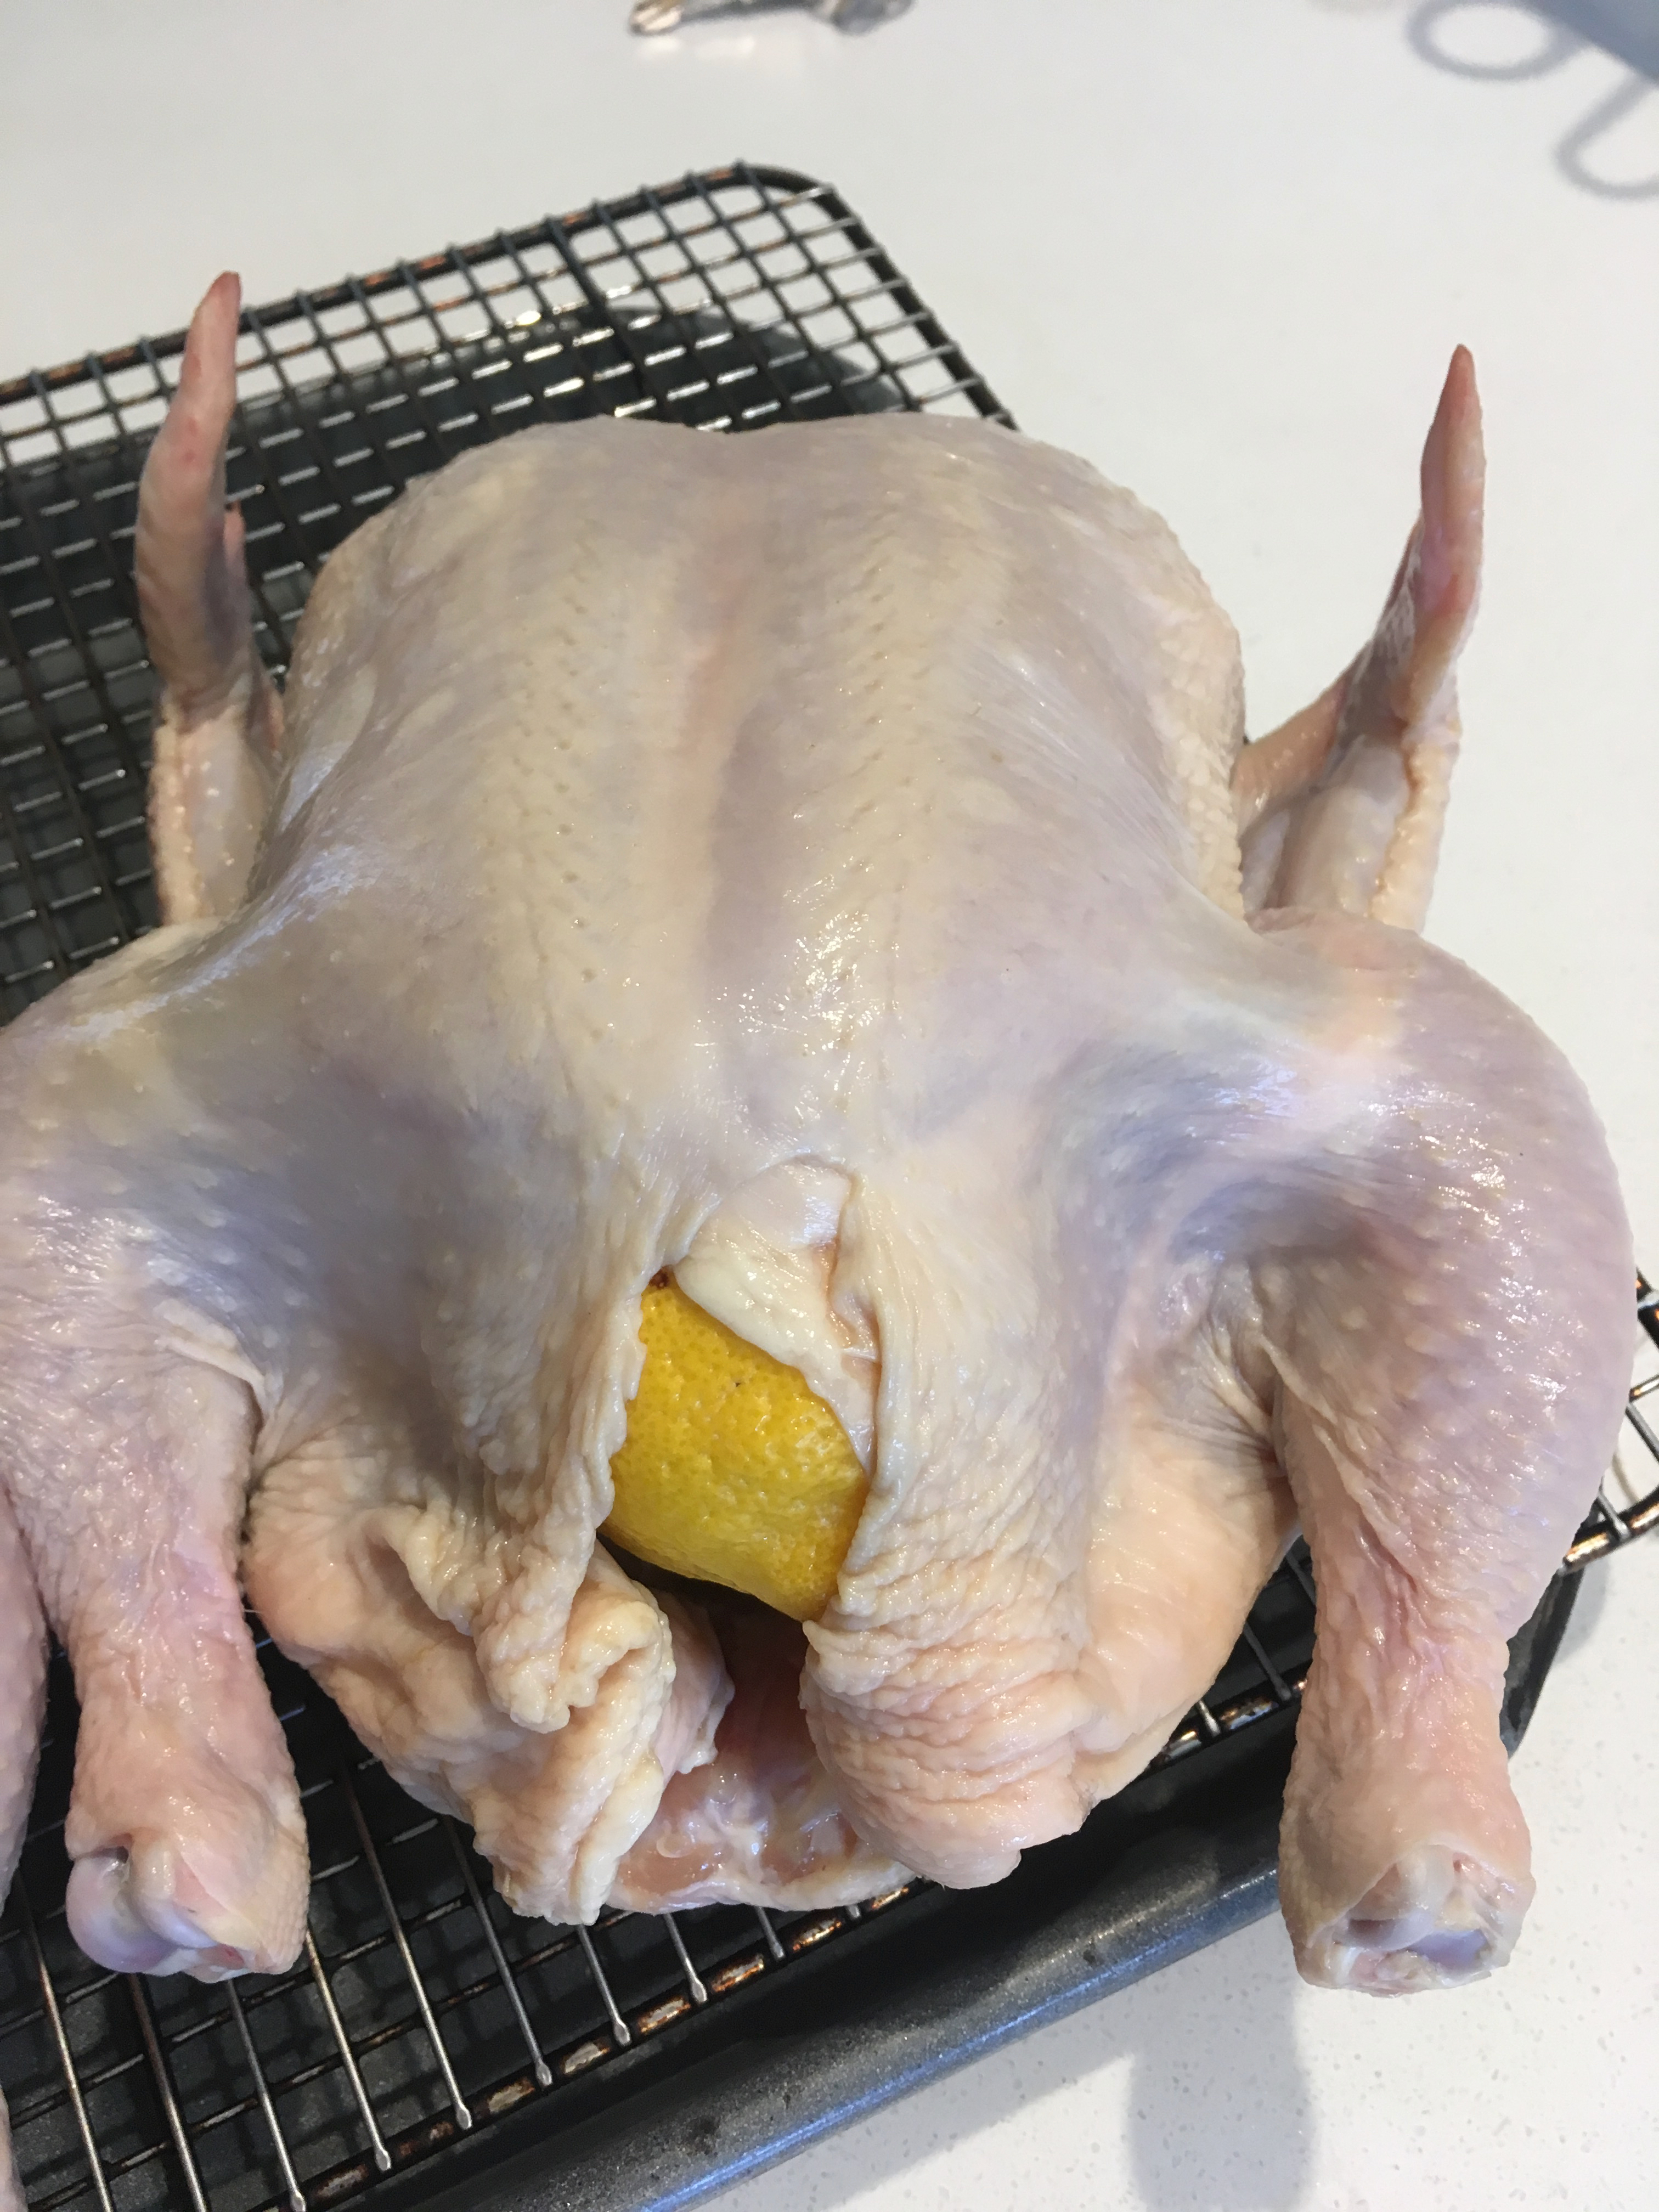
\includegraphics[width=0.25\textwidth]{\imageDir/\fileName/IMG_3213.jpg} \\
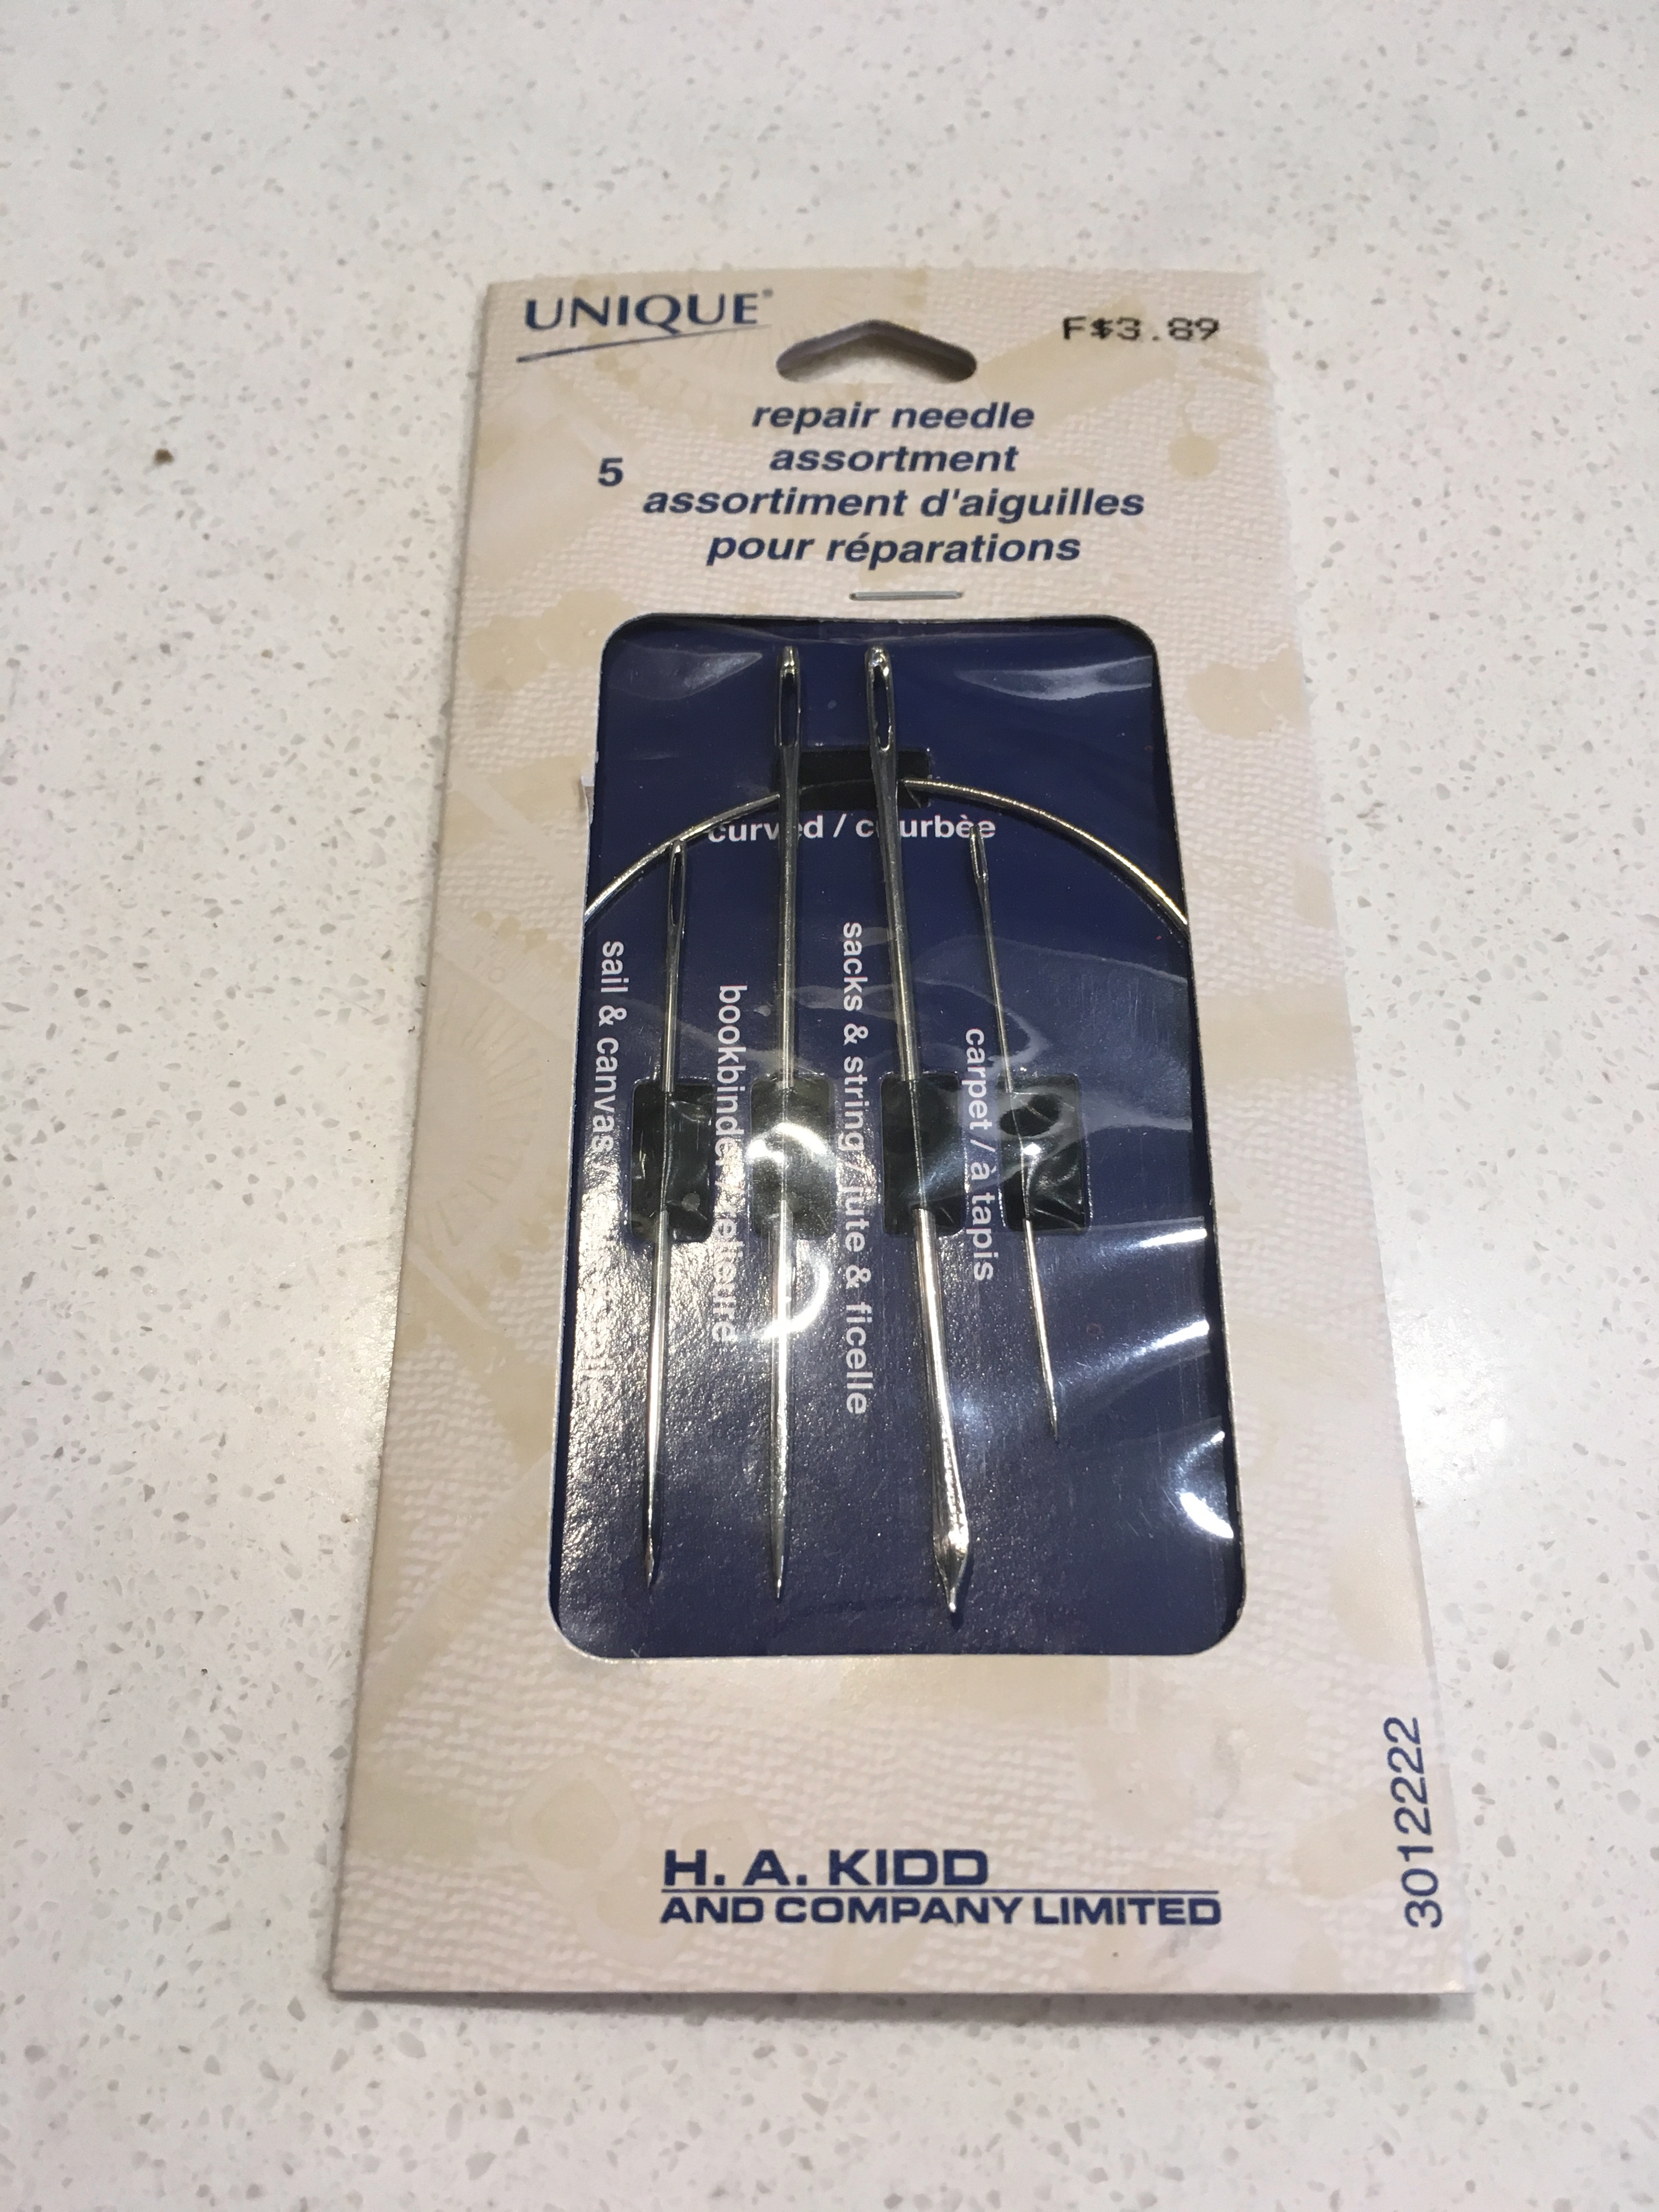
\includegraphics[width=0.25\textwidth]{\imageDir/\fileName/IMG_3206.jpg} &
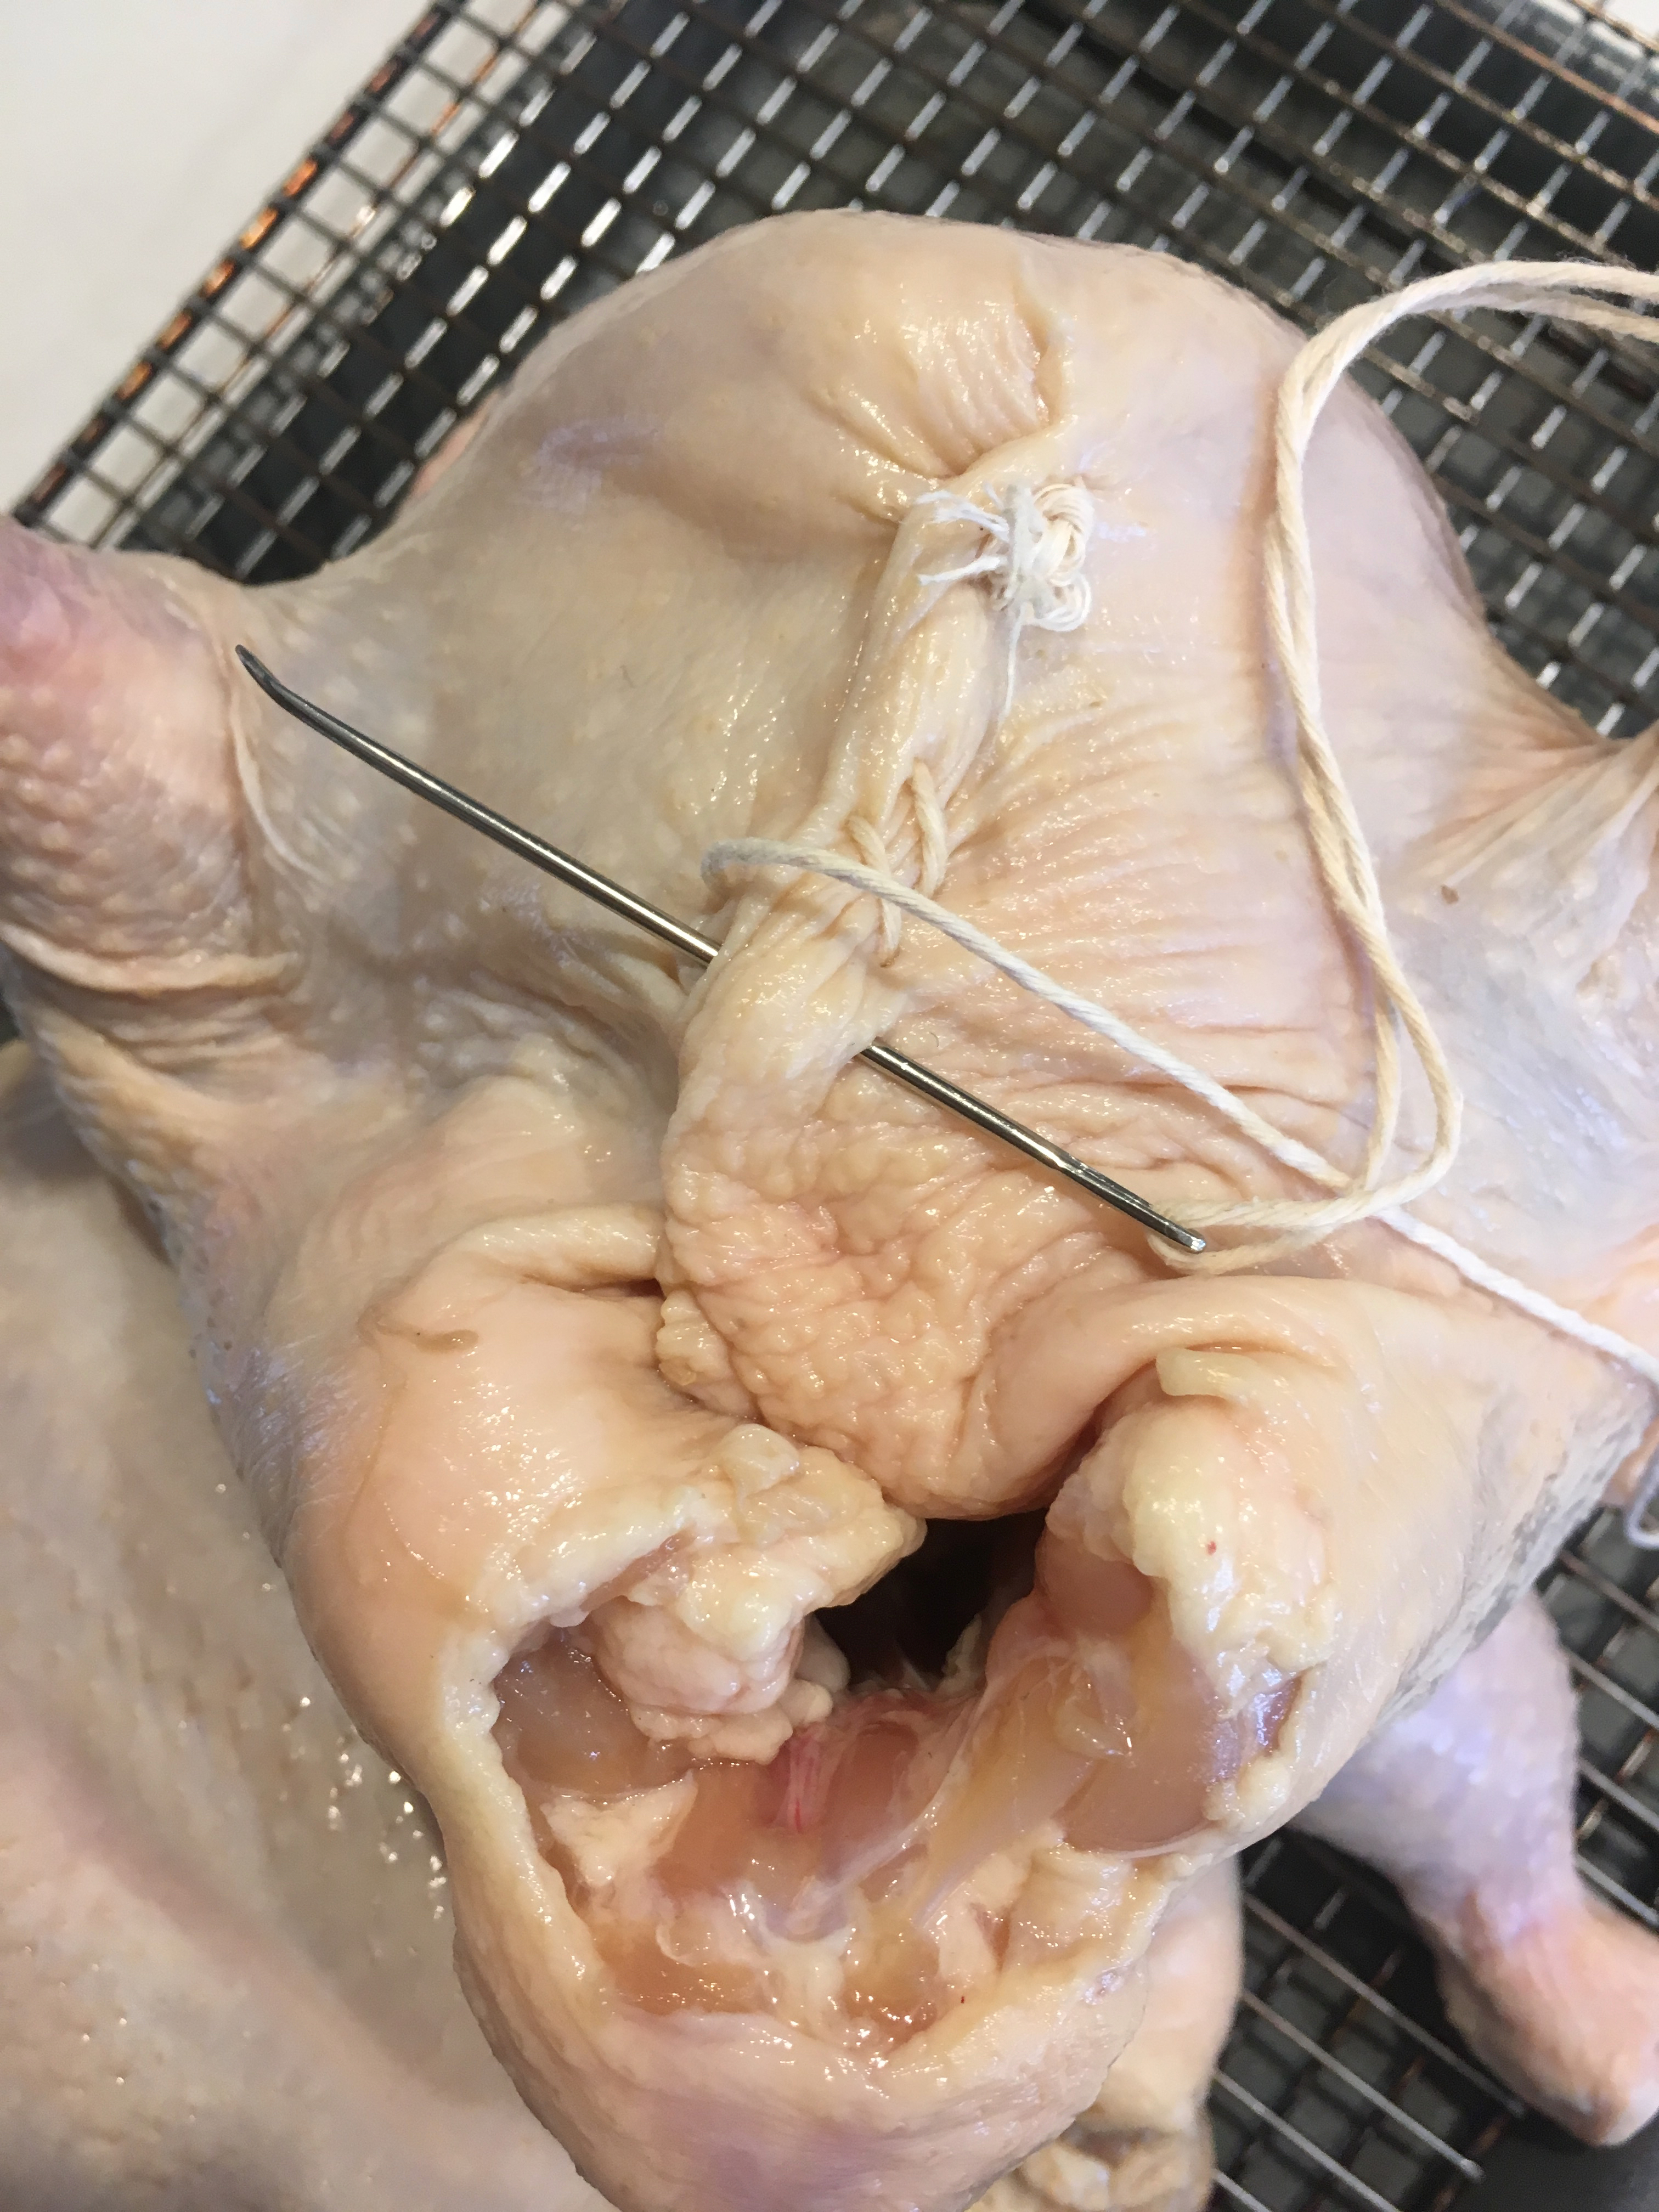
\includegraphics[width=0.25\textwidth]{\imageDir/\fileName/IMG_3214.jpg} &
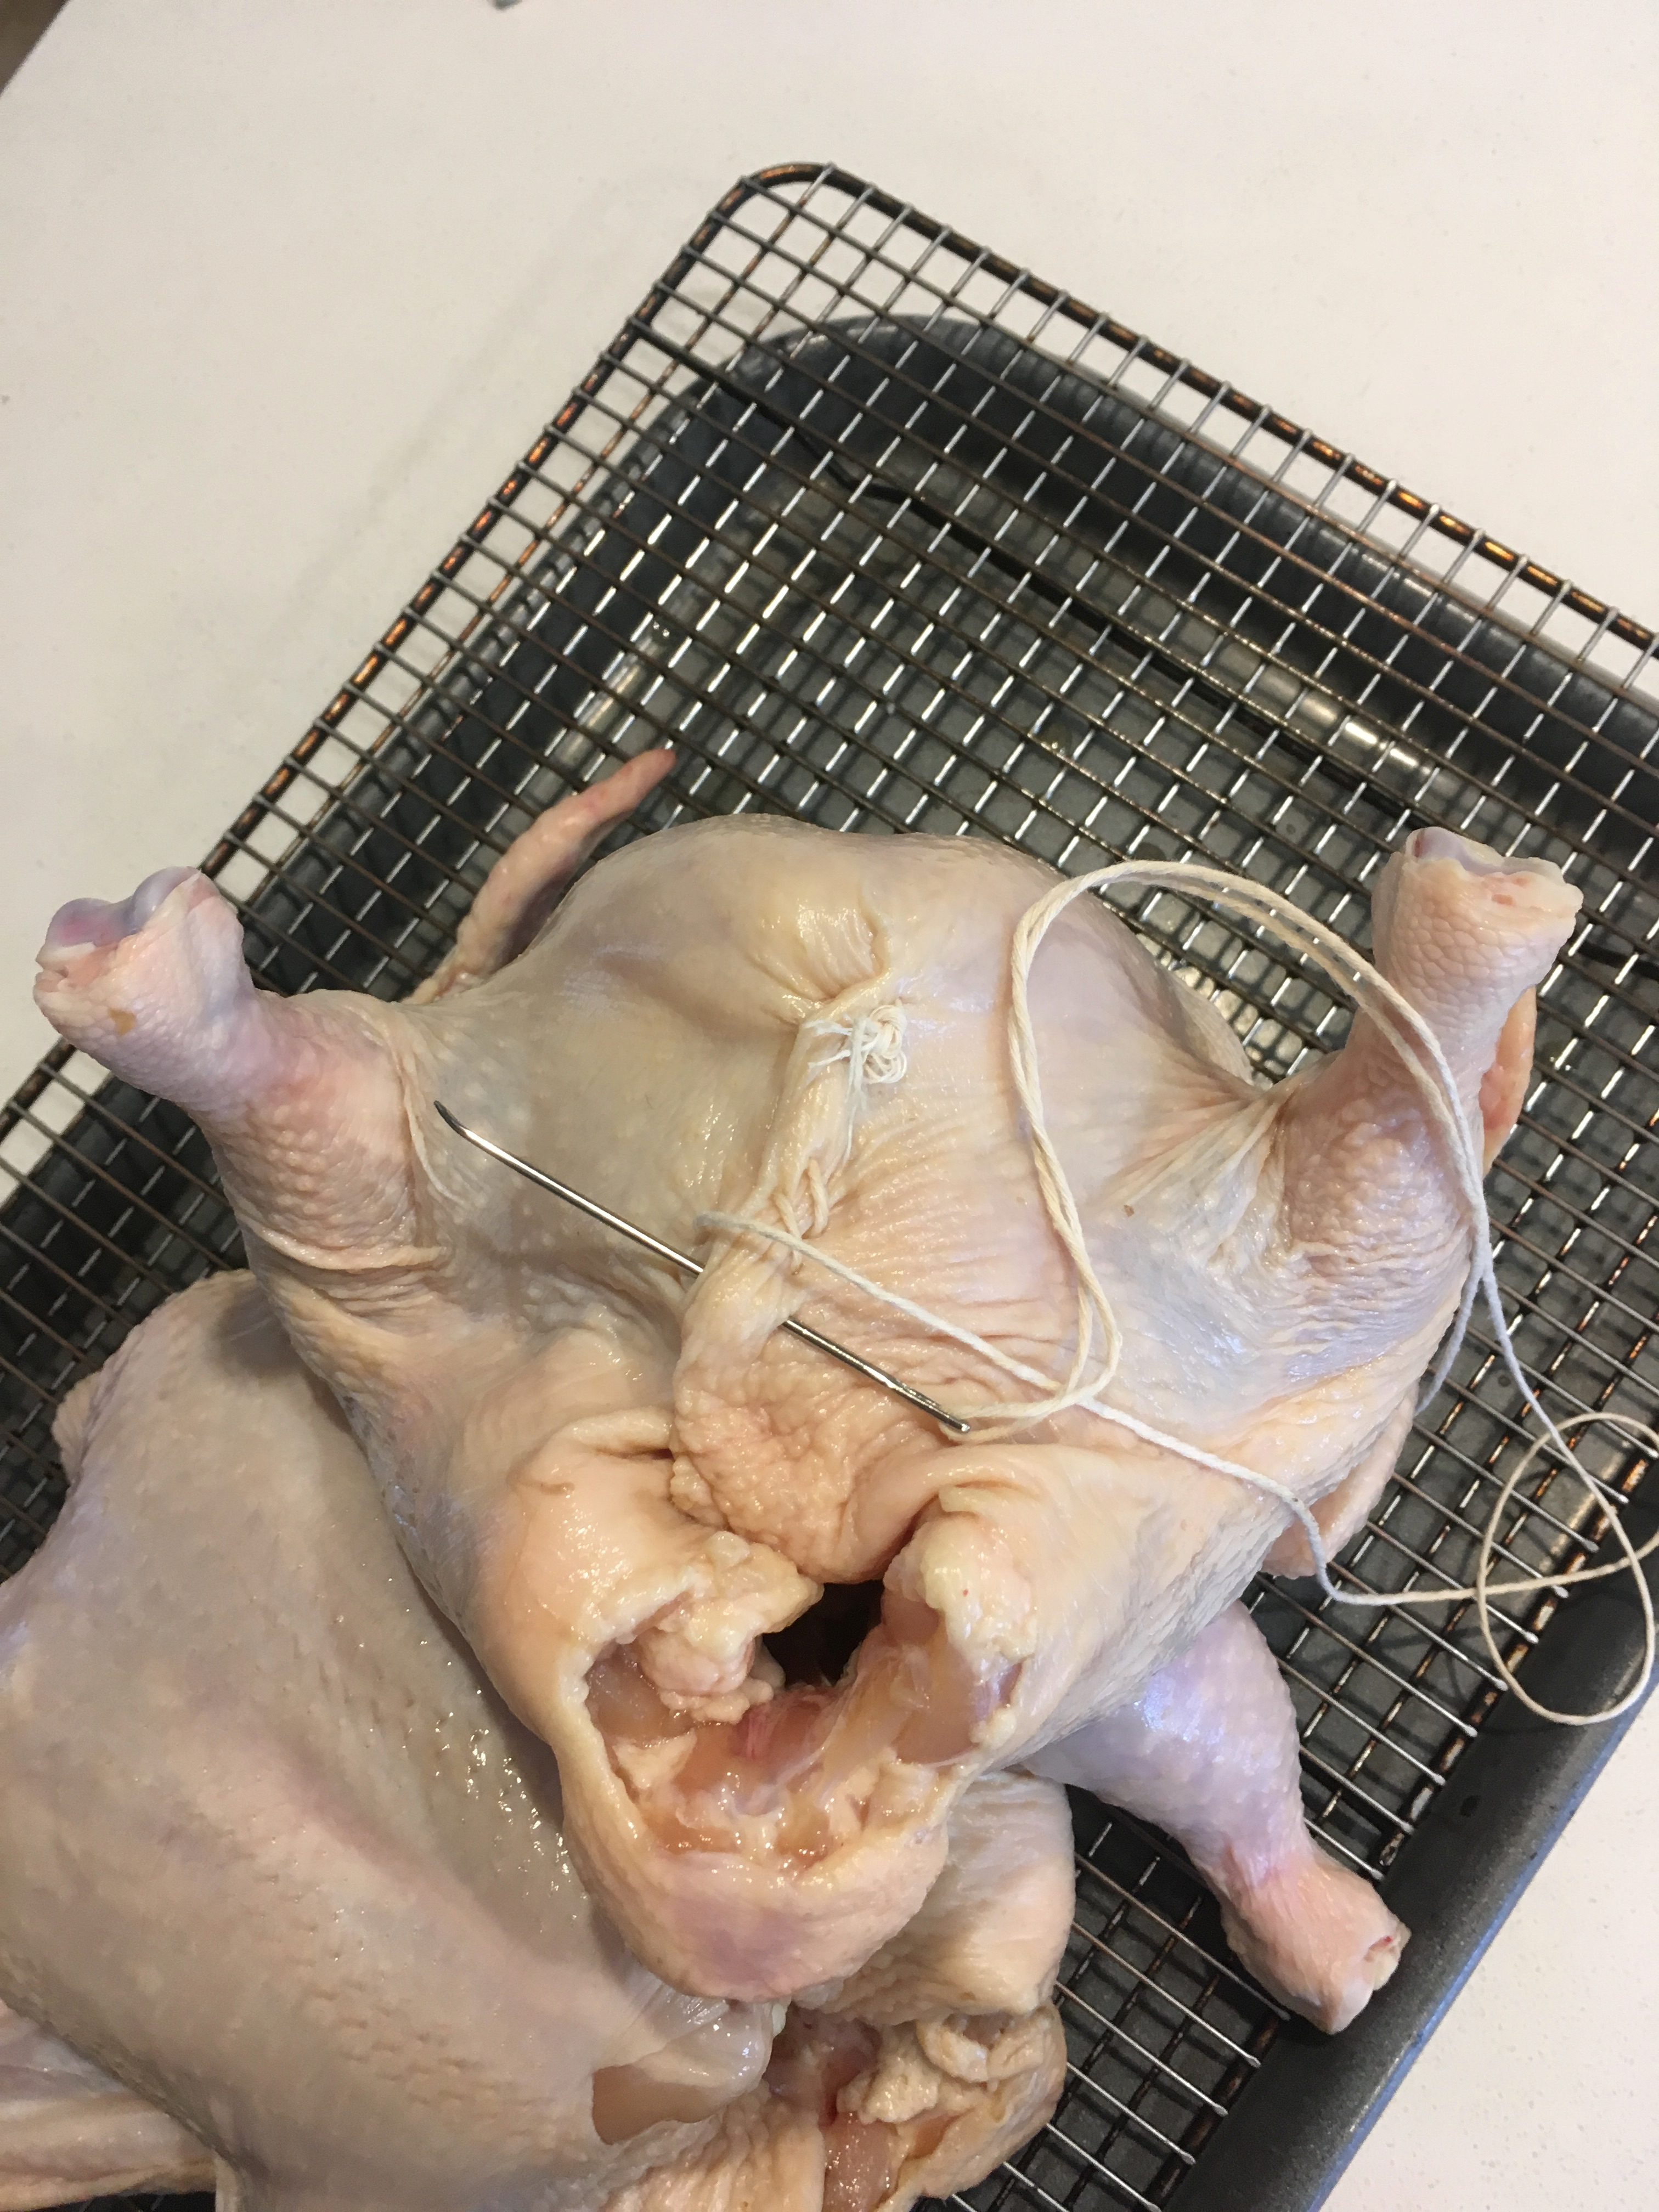
\includegraphics[width=0.25\textwidth]{\imageDir/\fileName/IMG_3216.jpg} \\
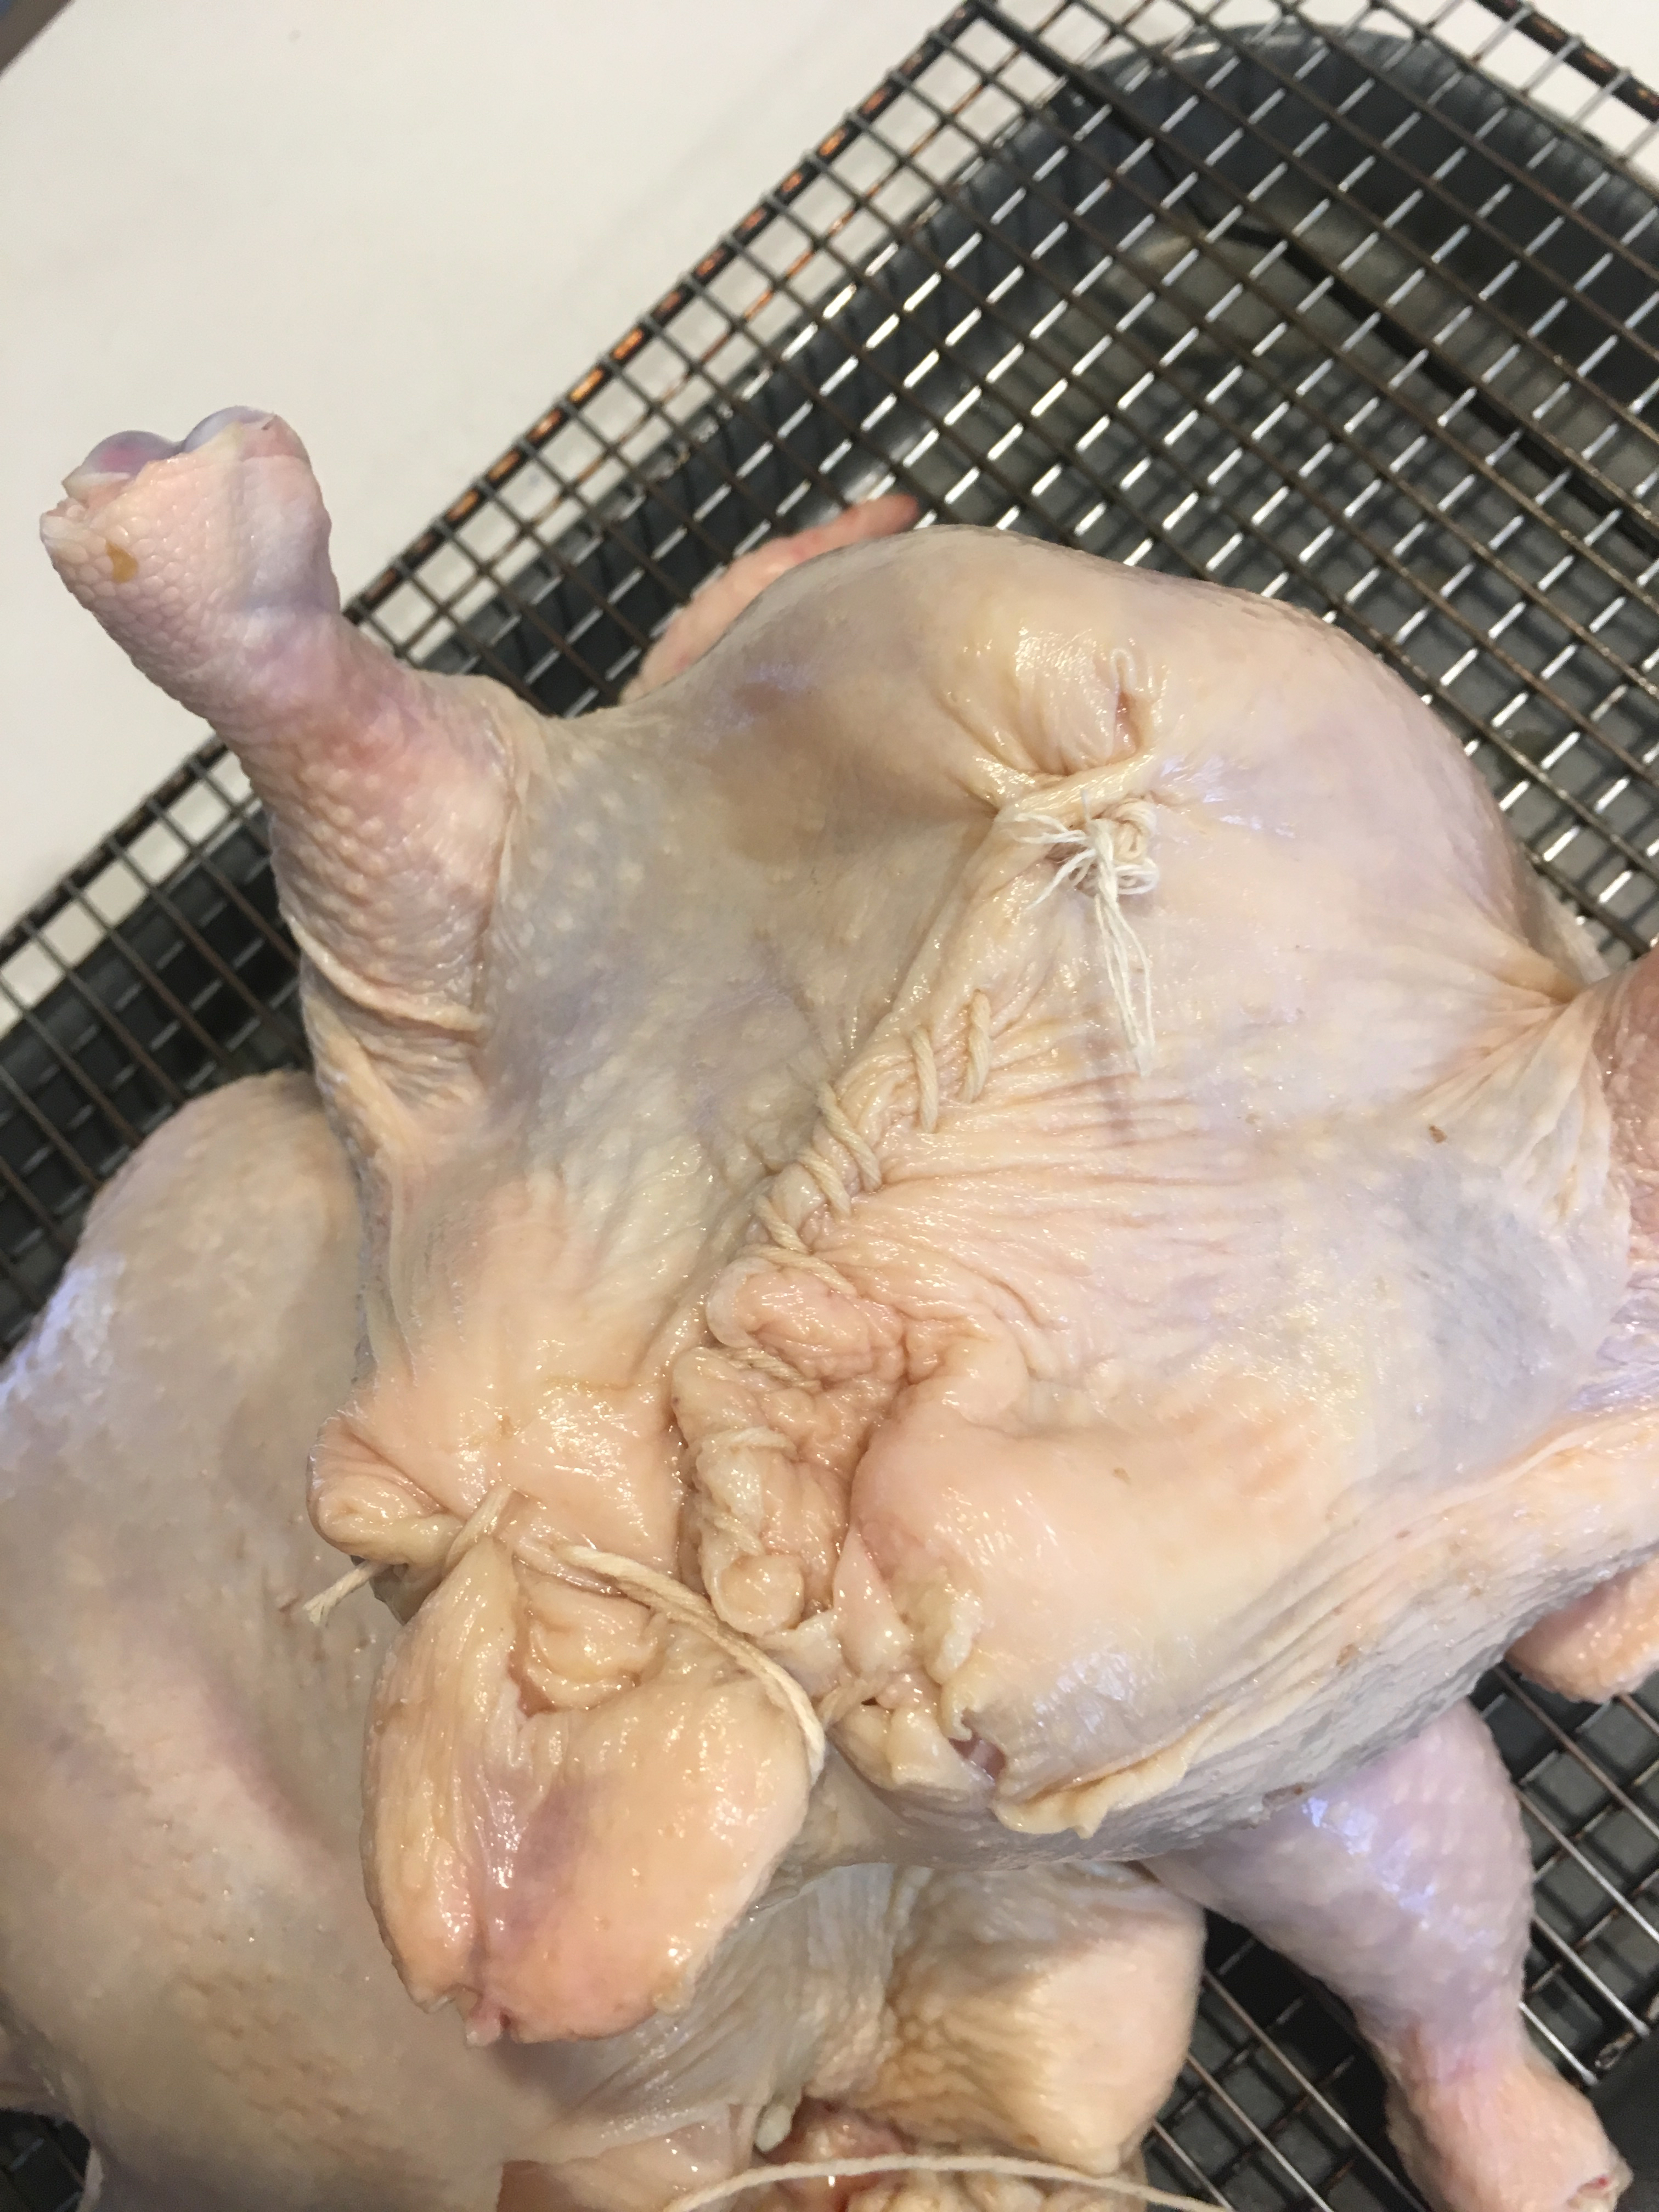
\includegraphics[width=0.25\textwidth]{\imageDir/\fileName/IMG_3217.jpg} &
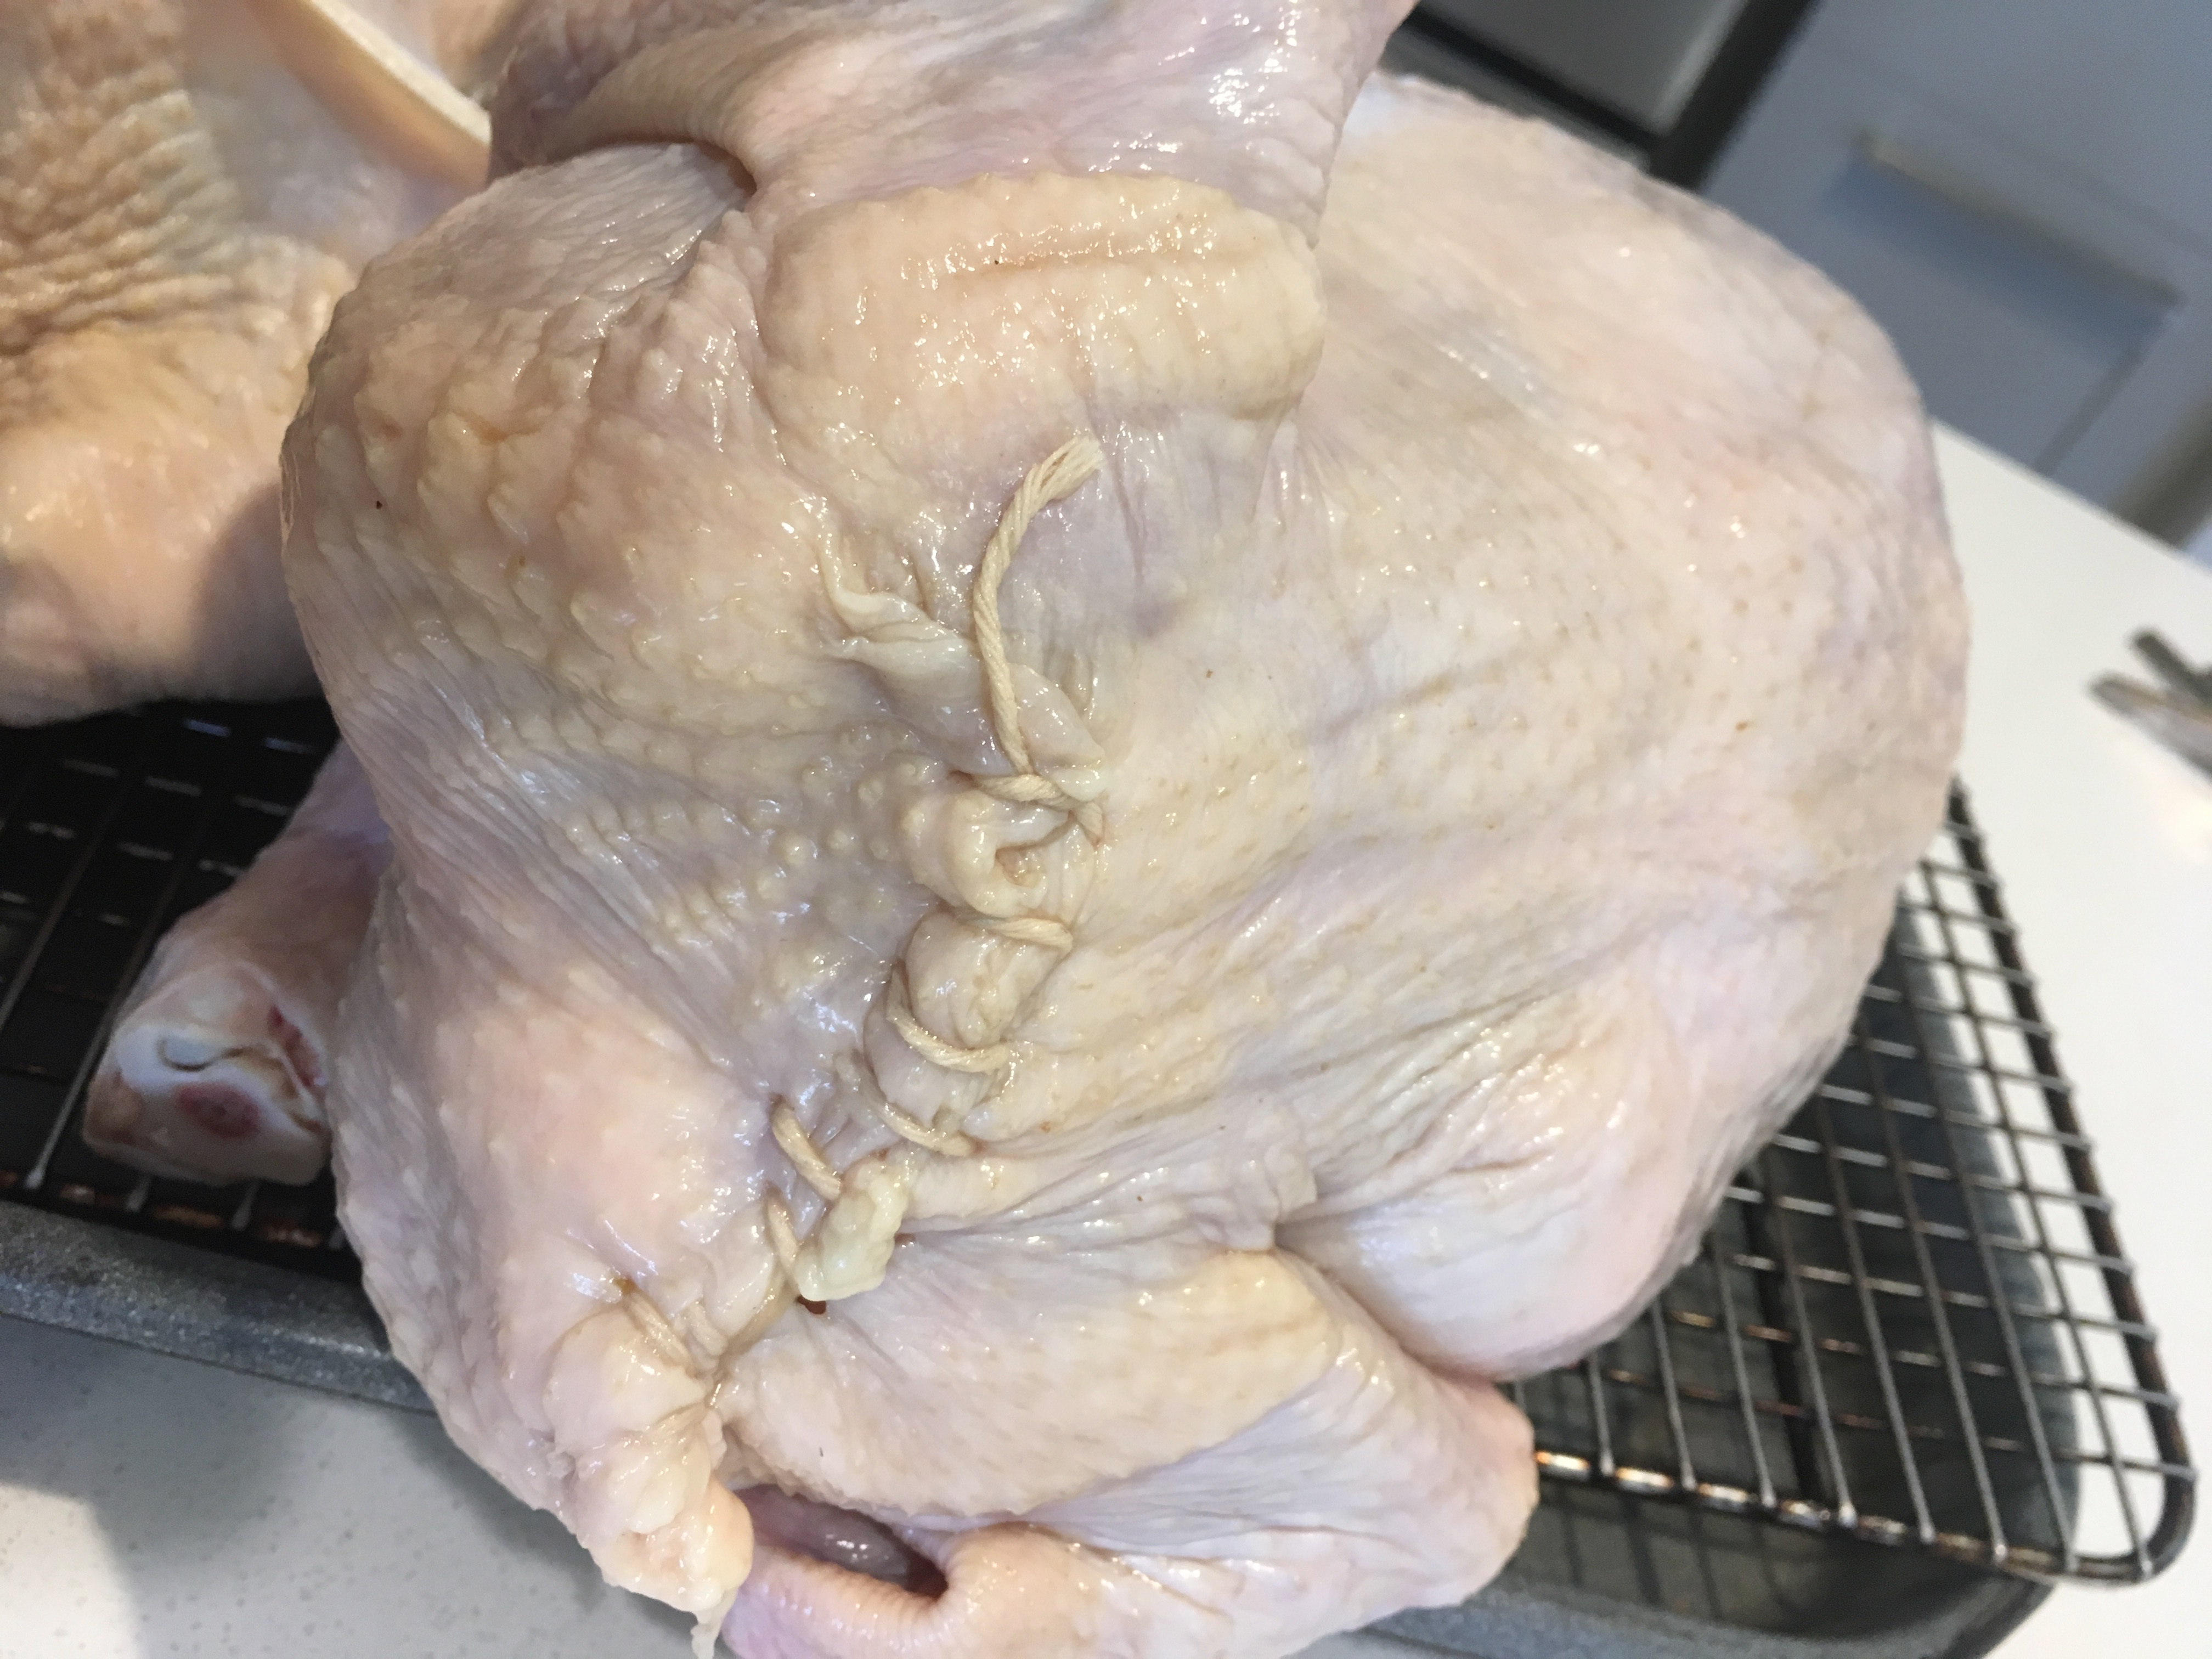
\includegraphics[width=0.25\textwidth]{\imageDir/\fileName/IMG_3218.jpg} &
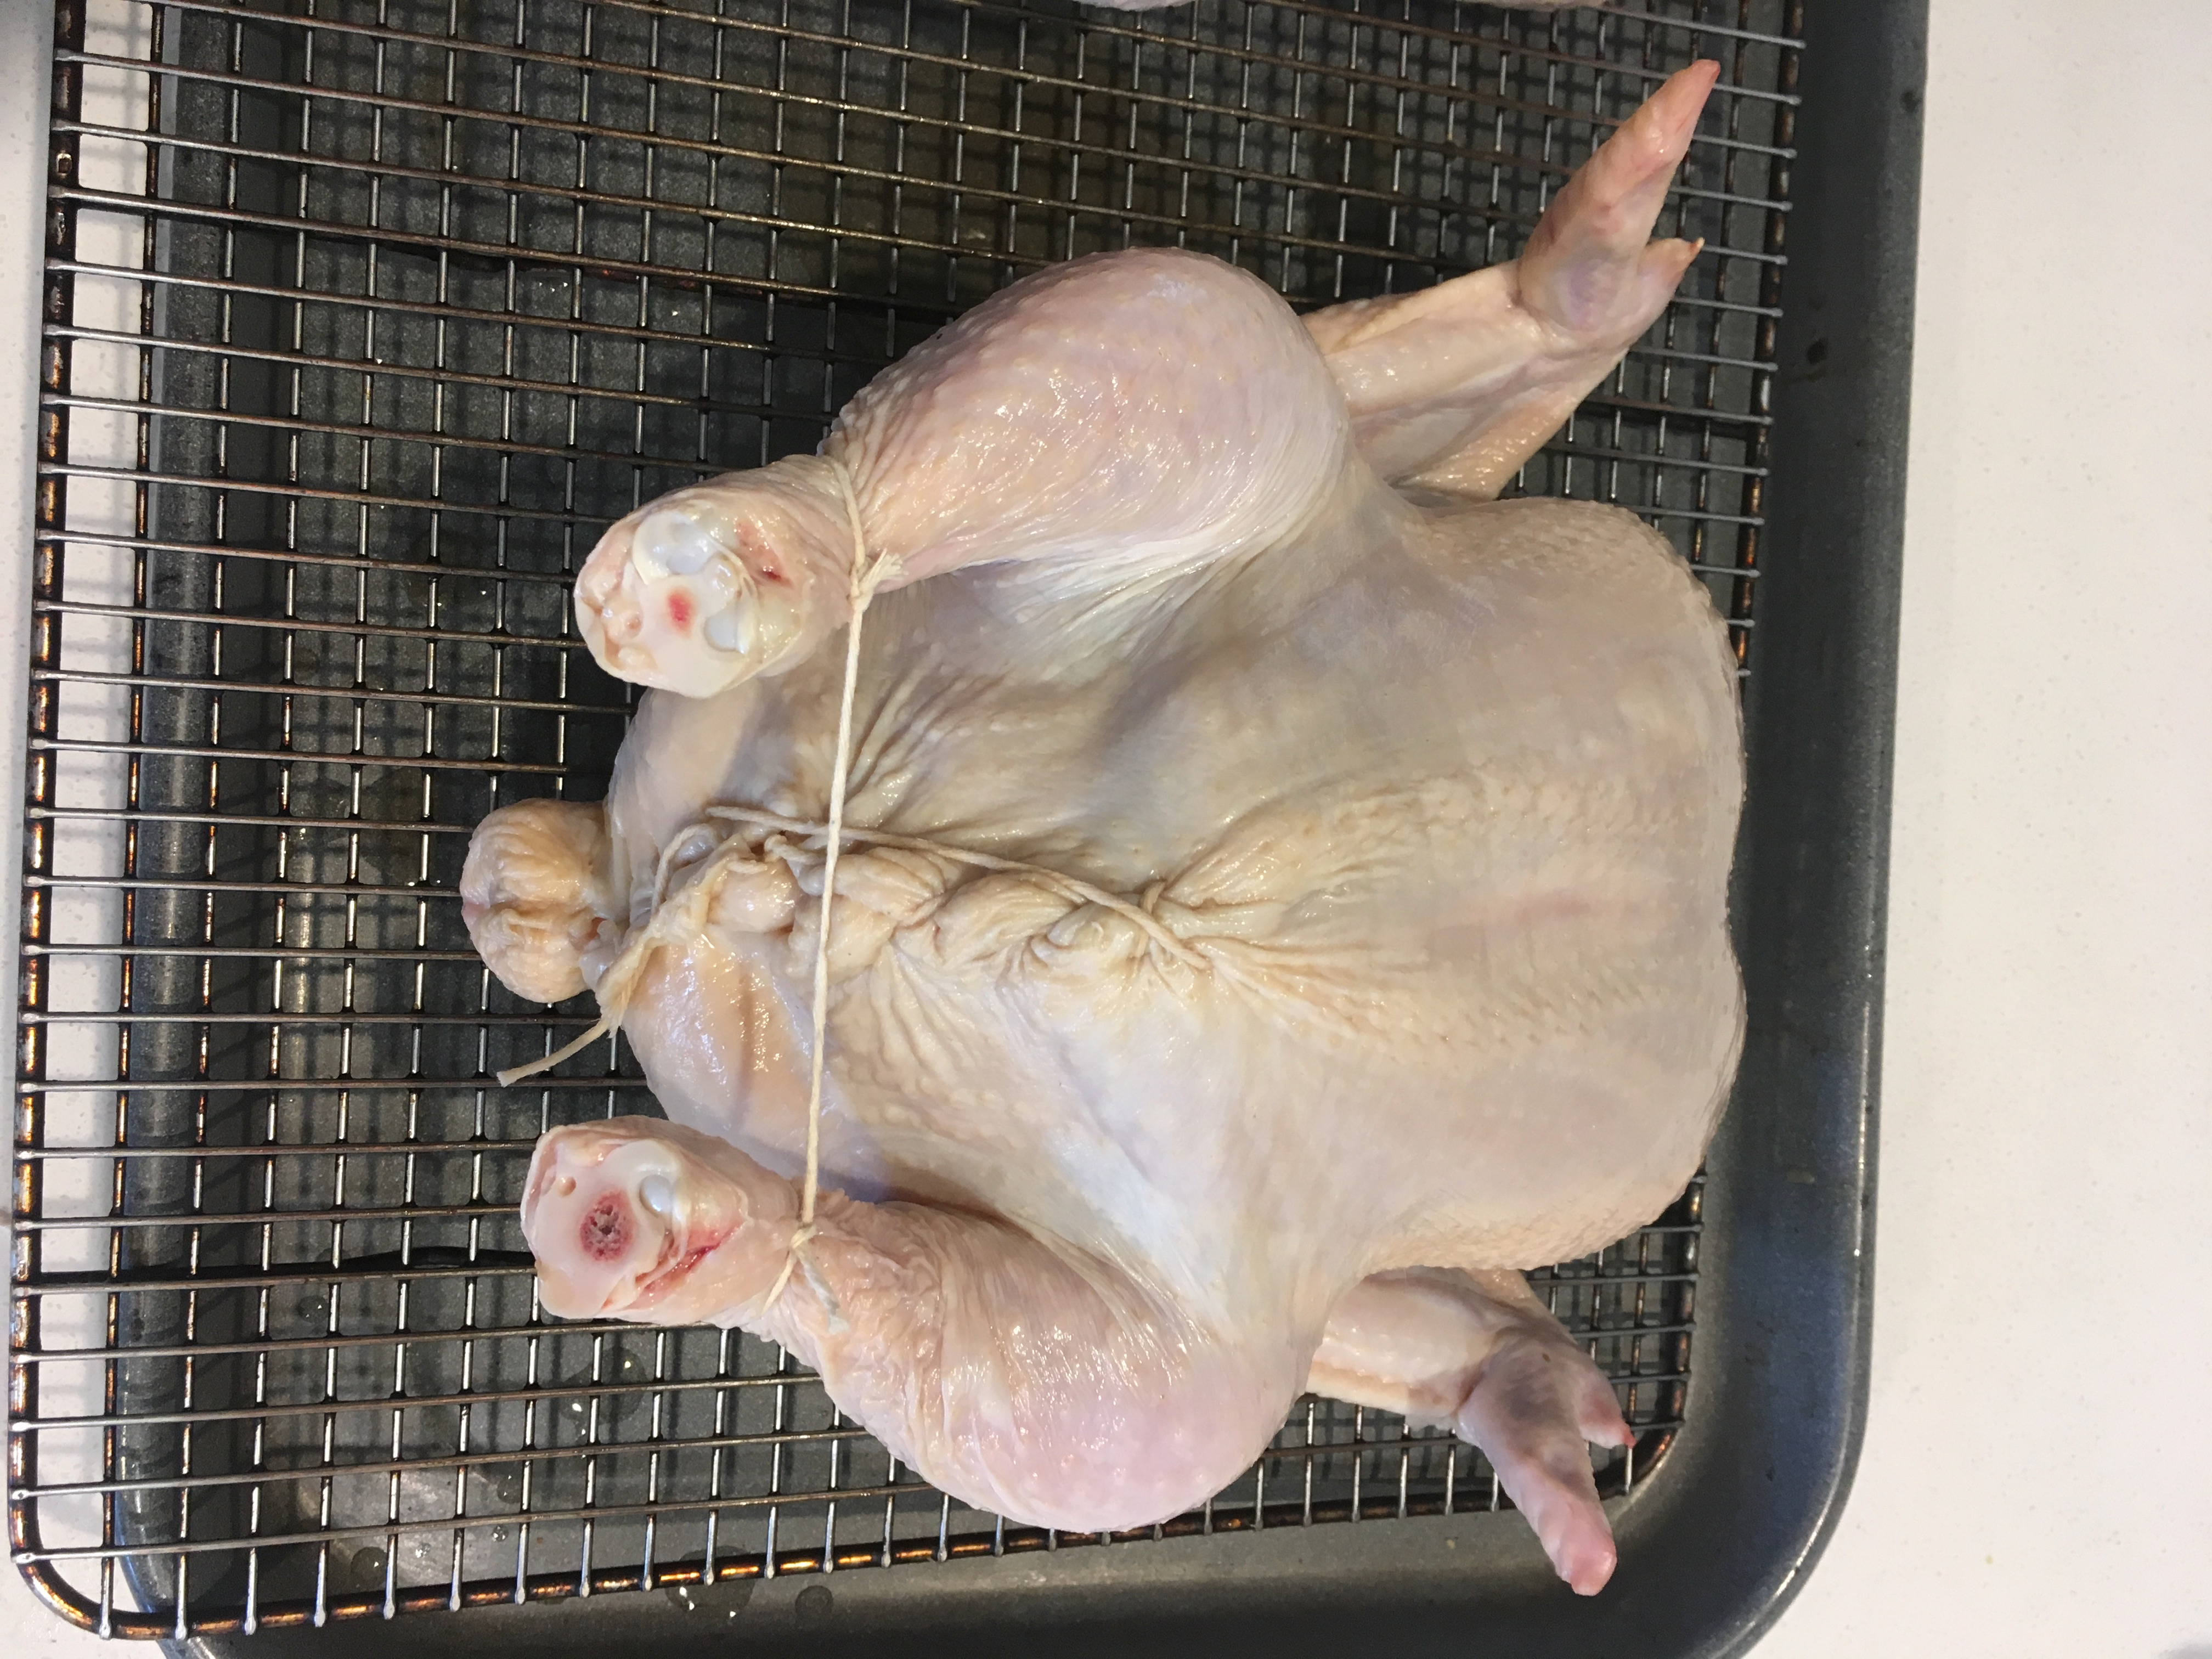
\includegraphics[width=0.25\textwidth]{\imageDir/\fileName/IMG_3219.jpg} \\
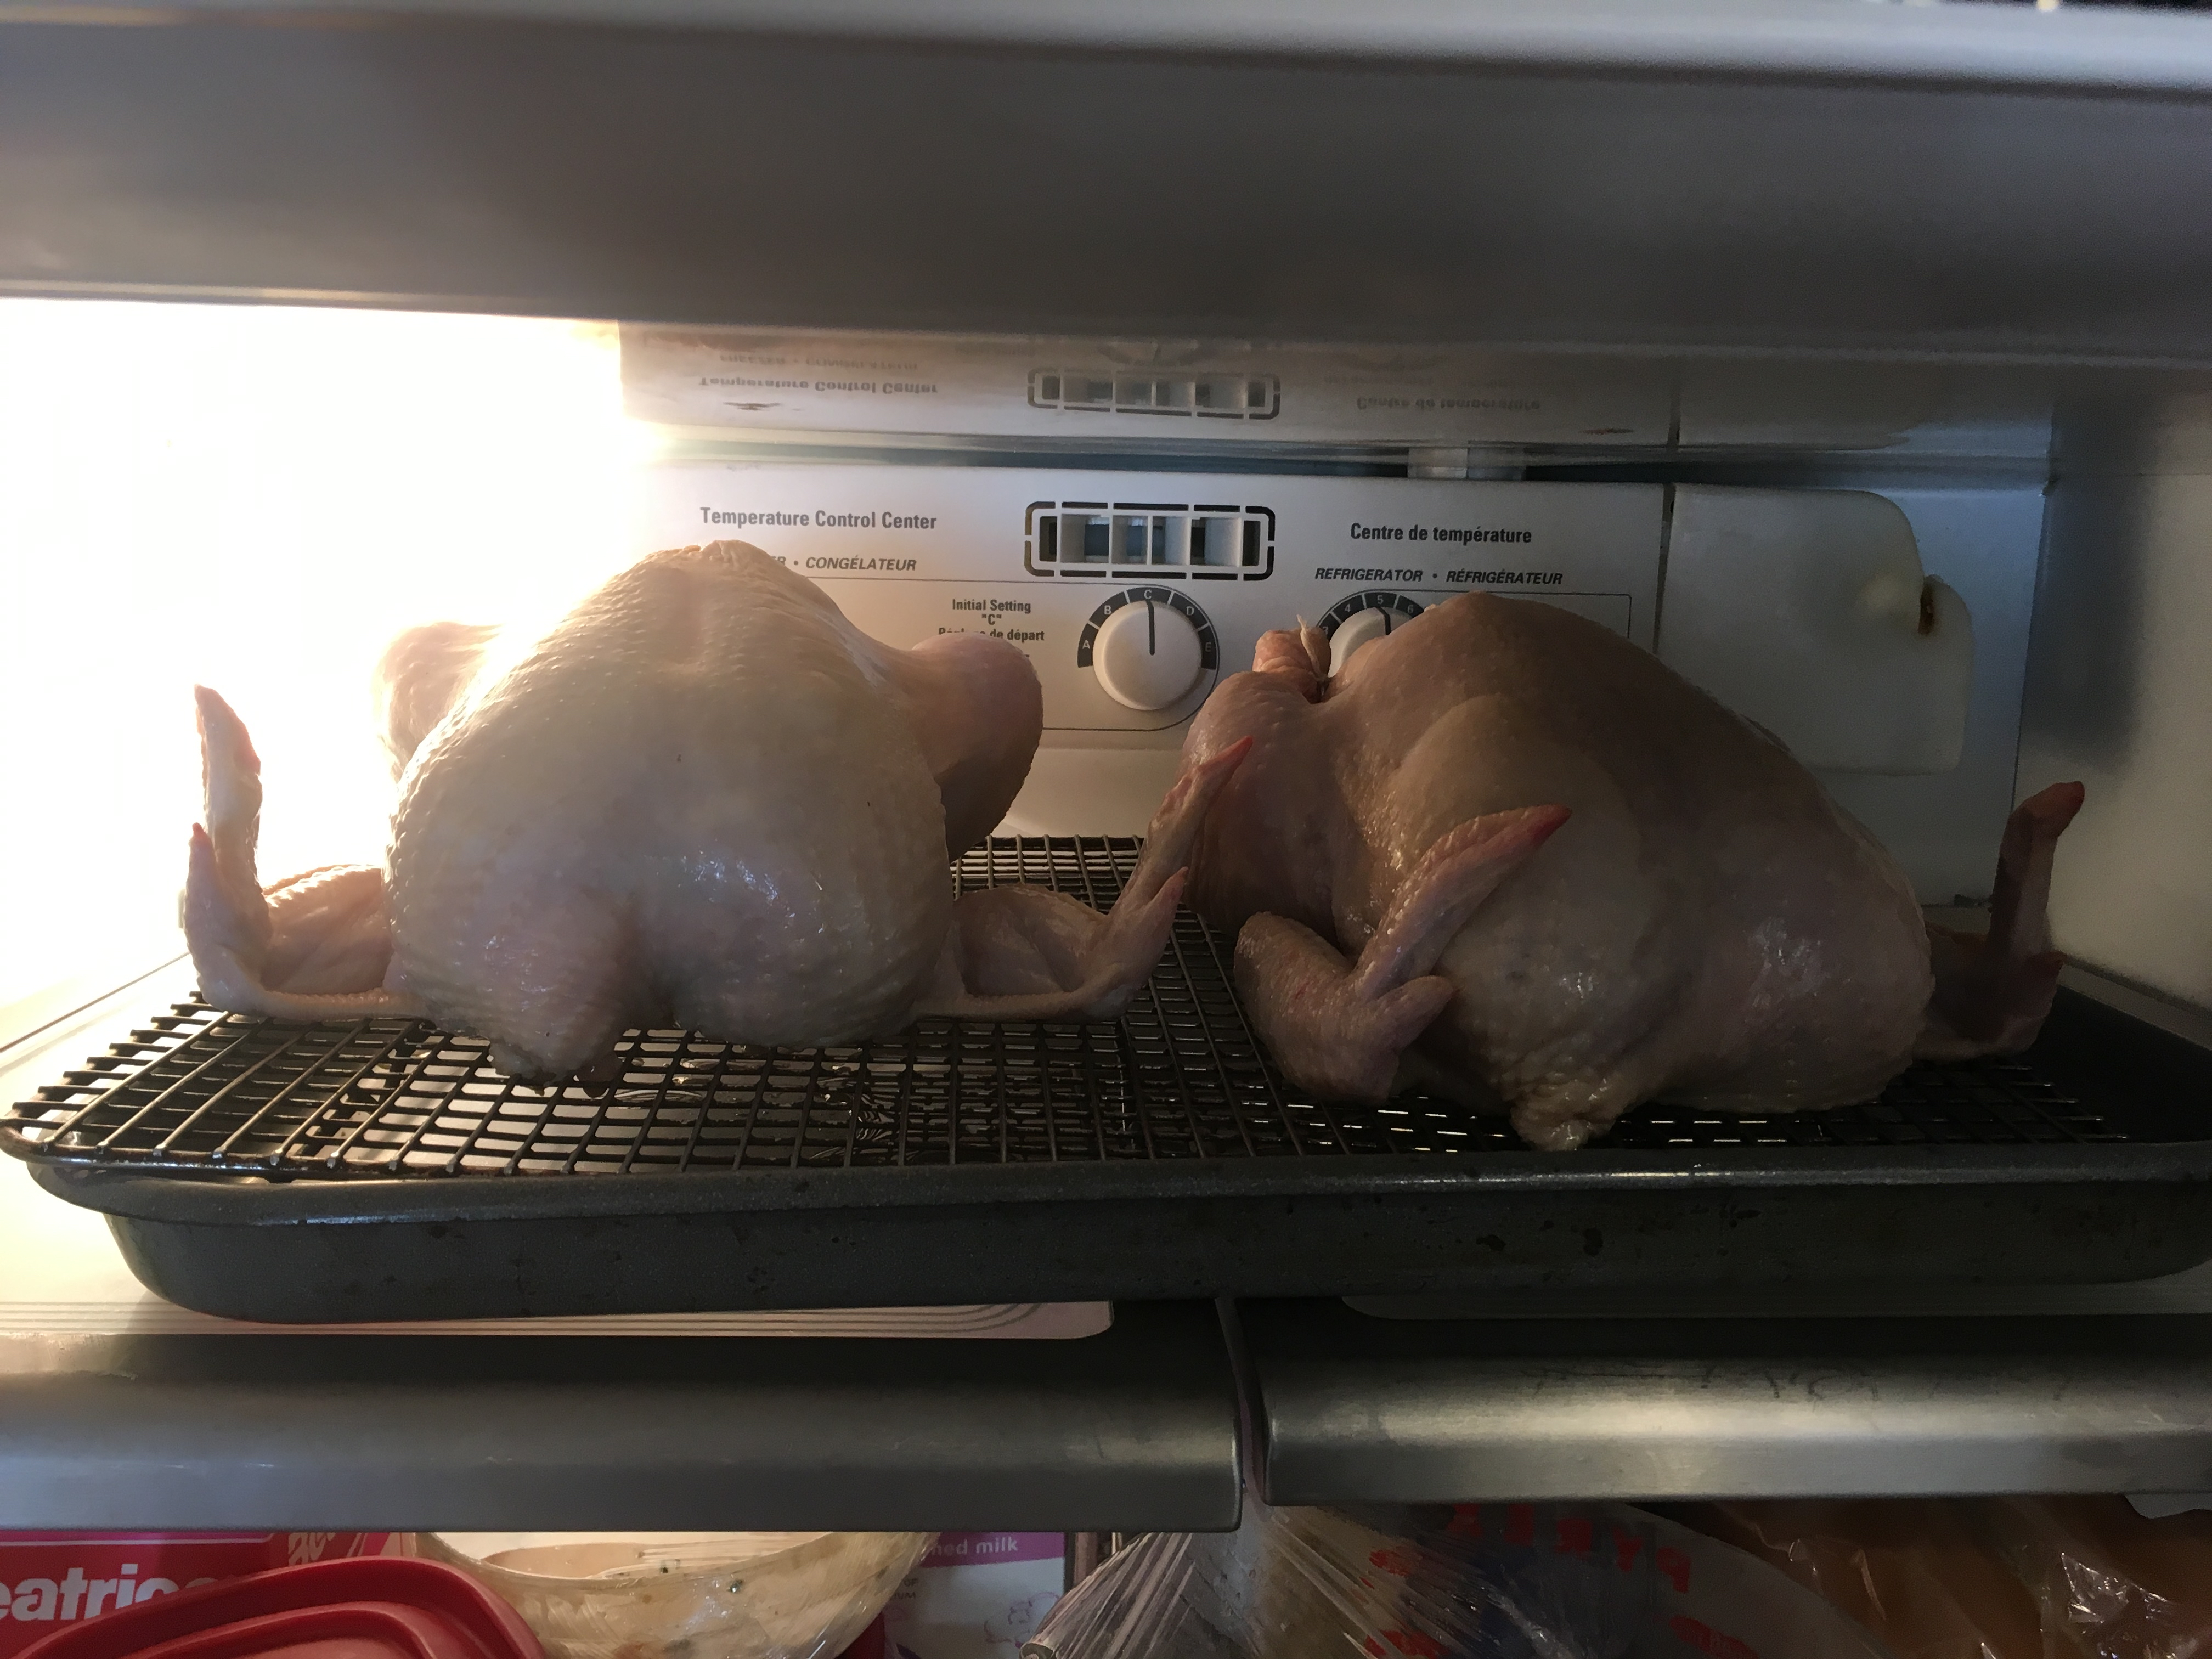
\includegraphics[width=0.25\textwidth]{\imageDir/\fileName/IMG_3220.jpg} &
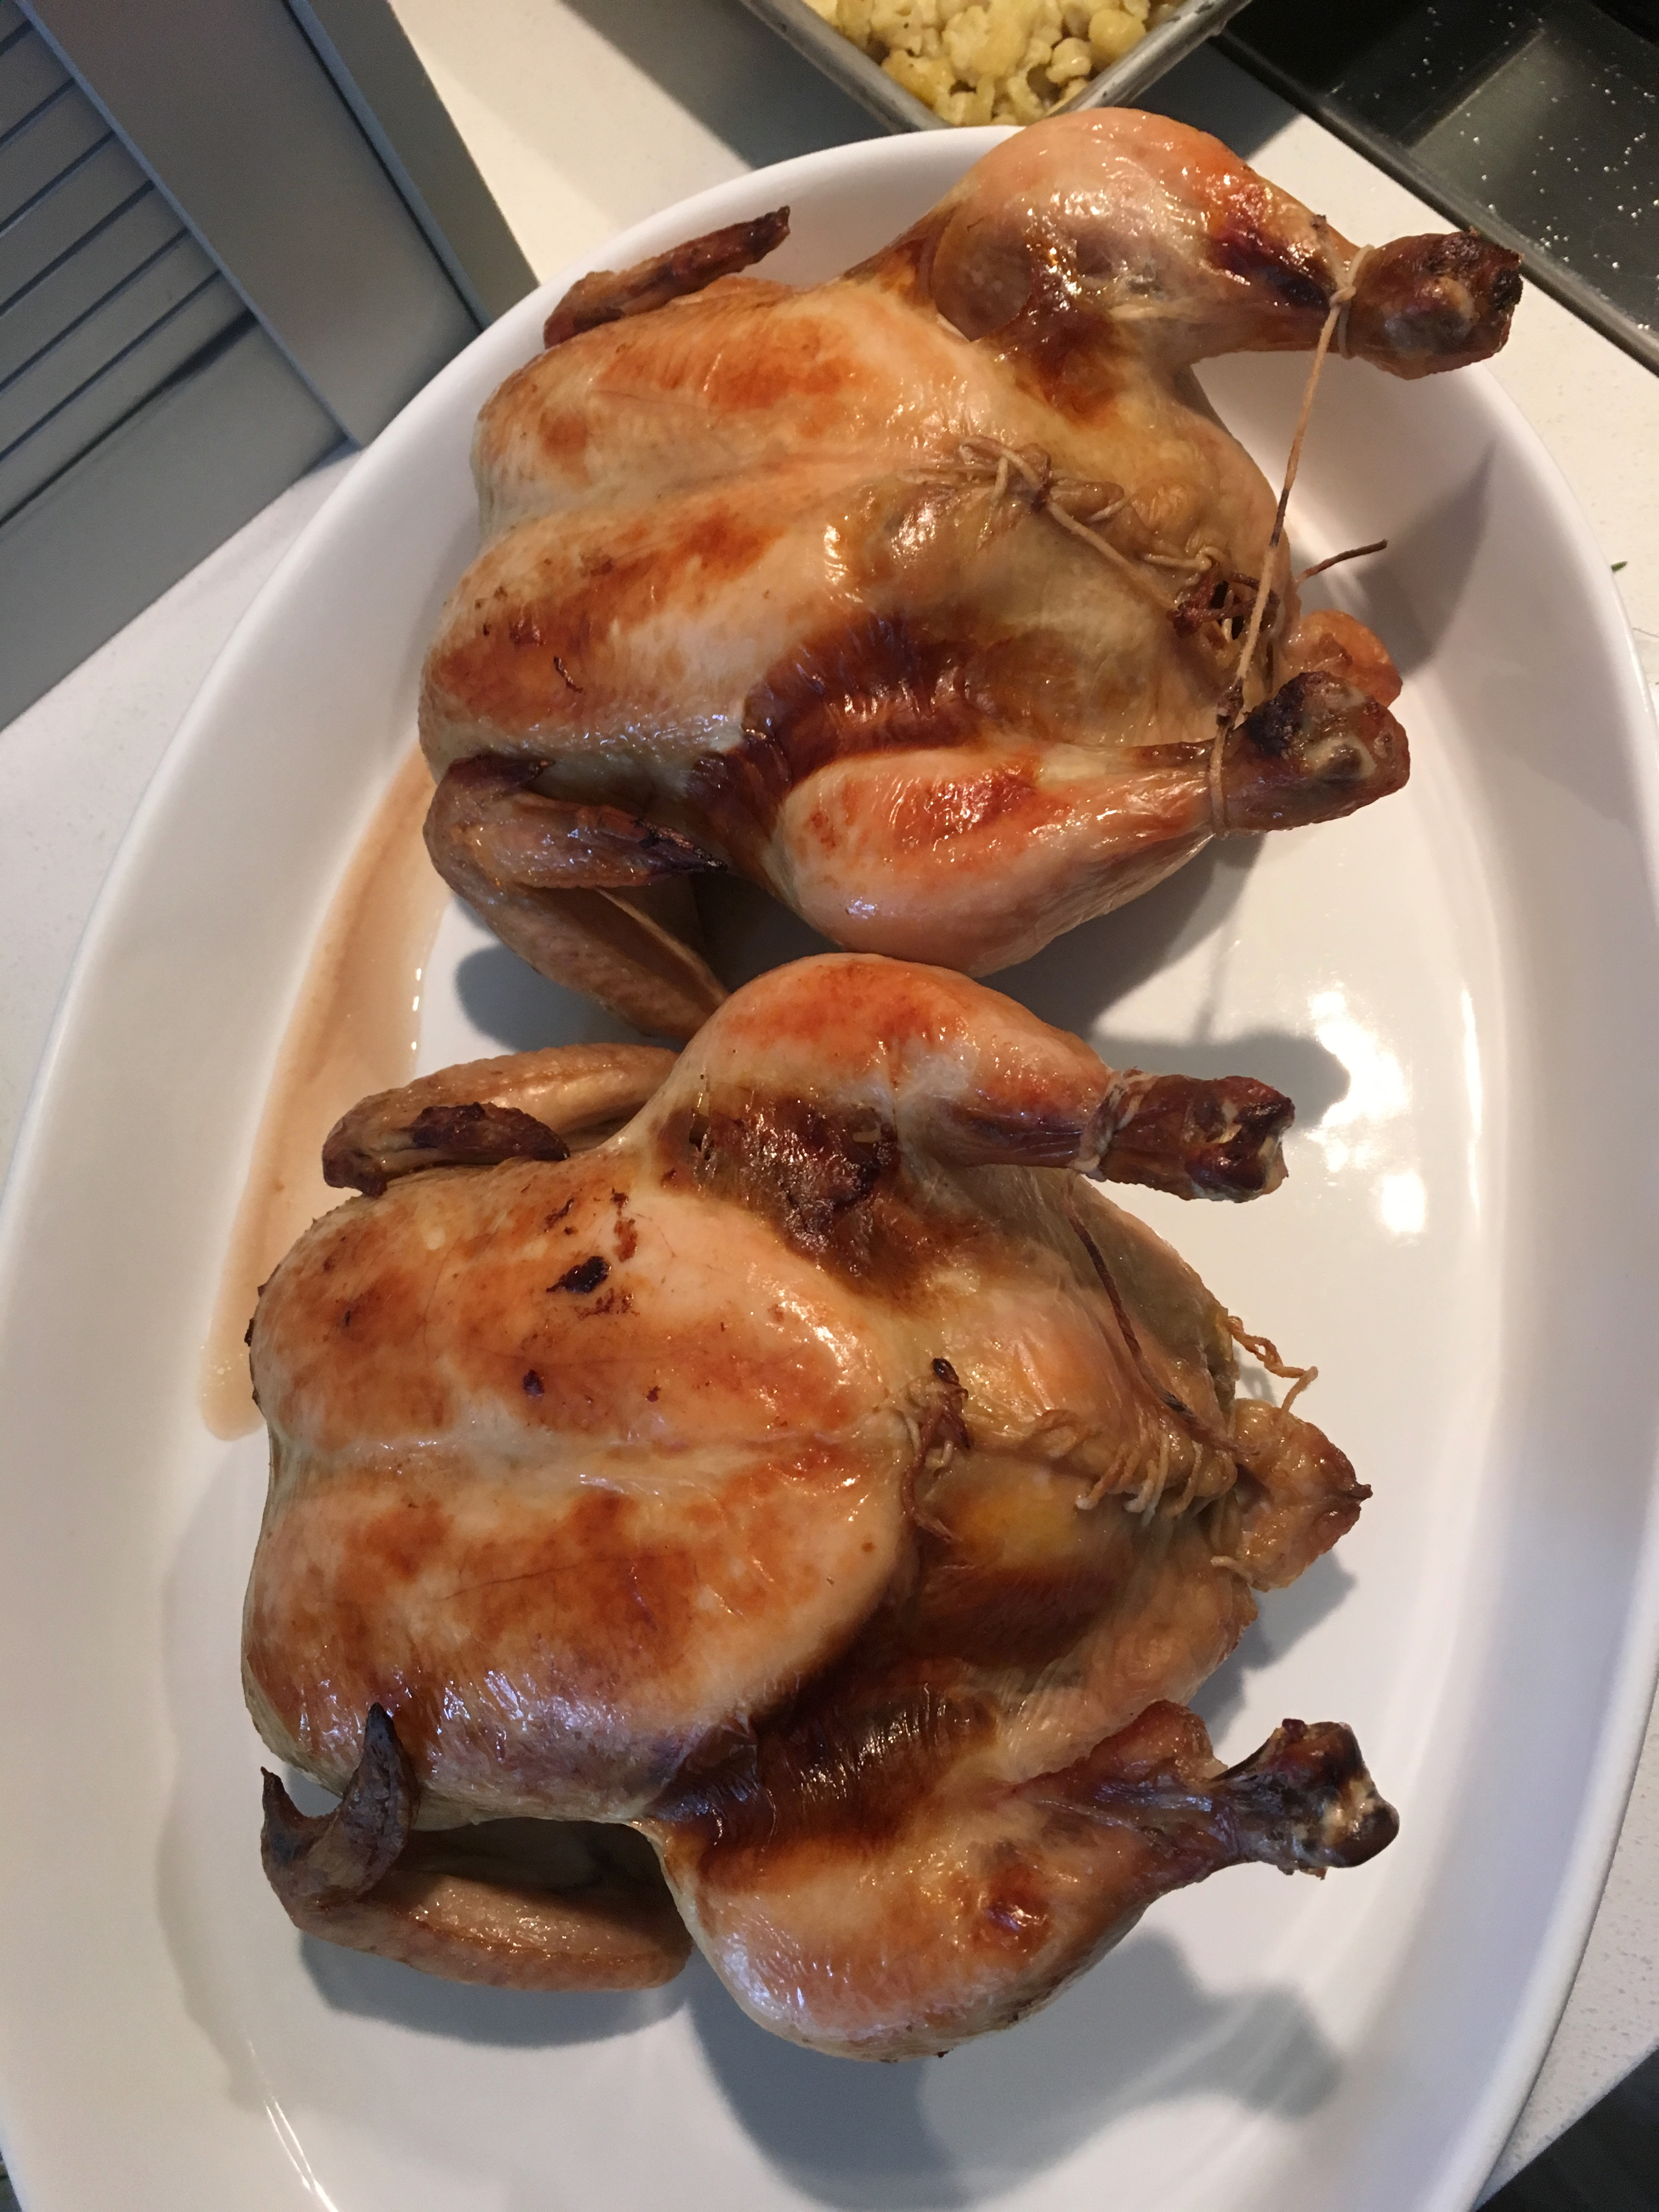
\includegraphics[width=0.25\textwidth]{\imageDir/\fileName/IMG_3228.jpg} \\
\end{tabular}
\end{table}


\end{document}



